%
% LSST Data Products Definition Document
%
% Maintained by Mario Juric <mjuric@lsst.org>
%
\documentclass[SE,lsstdraft,toc]{lsstdoc}

\usepackage{comment}
\usepackage{listings}

\excludecomment{changelog}
\excludecomment{todo}
\excludecomment{openissues}

\newcommand\x         {\hbox{$\times$}}

\newcommand{\annotate}[1]{{\color{magenta}\large\textbf{\emph{#1}}}}

% Environment for displaying the schema tables in
% a consistent manner. Two arguments are the
% caption and short caption that differ for each table.
% The third argument is the label to use for the table
\newenvironment{schema}[3]{%
\setlength\LTleft{0pt}
\setlength\LTright{\fill}
\begin{longtable}{p{0.2\textwidth}p{0.14\textwidth}p{0.14\textwidth}p{0.41\textwidth}}

% First header has a caption with a label
\caption[#1]{#2\label{#3}}\\

\hline \textbf{Name} & \textbf{Type} & \textbf{Unit} & \textbf{Description}\\ \hline
\endfirsthead

% Subsequent headers have the caption but no label
\caption[#1]{#2}\\

\hline \textbf{Name} & \textbf{Type} & \textbf{Unit} & \textbf{Description}\\ \hline
\endhead

\hline \multicolumn{4}{r}{\emph{Continued on next page}} \\
\endfoot

\hline\hline
\endlastfoot
}{%
\hline
\end{longtable}
}


\title[DPDD]{Data Products Definition Document}

\author{
M. Juri\'c,
T.~Axelrod, A.C.~Becker, J.~Becla, E.~Bellm, J.F.~Bosch, D.~Ciardi,
A.J.~Connolly,  G.P.~Dubois-Felsmann, F.~Economou, M.~Freemon,
M.~Gelman, M.~Graham, \v{Z}.~Ivezi\'c, T.~Jenness,  J.~Kantor, K.S.~Krughoff,
K-T~Lim,  R.H.~Lupton, F.~Mueller, D.~Nidever, M.~Patterson, D.~Petravick, D. Shaw,
C.~Slater, M.~Strauss, J.~Swinbank, J.A.~Tyson, M.~Wood-Vasey, and X.~Wu
}

\date{\today}

\setDocRef{LSE-163}
\setDocCurator{Mario Juri\'c}
\setDocUpstreamLocation{\url{https://github.com/lsst/LSE-163}}

\setDocAbstract{%
This document describes the data products and processing services to be delivered by the Large Synoptic Survey Telescope (LSST).

The LSST will deliver three levels of data products and services. \textbf{Level 1} (nightly) data products will include images, difference images, catalogs of sources and objects detected in difference images, and catalogs of Solar System objects. Their primary purpose is to enable rapid follow-up of time-domain events. \textbf{Level 2} (annual) data products will include well calibrated single-epoch images, deep coadds, and catalogs of objects, sources, and forced sources, enabling static sky and precision time-domain science. \textbf{Level 3} (user-created) data product services will enable science cases that greatly benefit from co-location of user processing and/or data within the LSST Archive Center. LSST will also devote 10\% of observing time to programs with special cadence. Their data products will be created using the same software and hardware as Levels 1 and 2. All data products will be made available using user-friendly databases and web services.

%This is an \textbf{internal draft} and a work in progress. \textbf{It should not be circulated widely until this notice is removed.}
}

%
%   Revision history
%
% OLDEST FIRST: VERSION, DATE, DESCRIPTION, OWNER NAME
\setDocChangeRecord{%
\addtohist{1}{2013-10-07}{Initial release}{Mario Juric}
\addtohist{2}{2016-09-26}{Implementation of LCR-758 Update Data Products Definition Document, LSE-163}{Gregory Dubois-Felsmann (LCR), Tim Jenness (document), Robert McKercher (Docushare)}
\addtohist{3.0}{2017-07-03}{Implementation of LCR-962. Reference LSE-61 requirements. Minor clean ups.}{Tim Jenness}
}

\begin{document}
\maketitle

% Turn off page numbering for the preface
\pagenumbering{gobble}

\section*{Preface}

The purpose of this document is to describe the data products produced by the Large Synoptic Survey Telescope (LSST).

To a future LSST user, it should clarify what catalogs, image data, software, and services they can expect from LSST. To LSST builders, it provides direction on how to flow down the LSST System Requirements Document to system design, sizing, budget and schedule as they pertain to the data products.

Though under strict change control, this is a \textbf{\emph{living document}}. LSST will undergo a period of construction  and commissioning lasting no less than seven years, followed by a decade of survey operations. To ensure their continued scientific adequacy, the designs and plans for LSST Data Products will be periodically reviewed and updated.

\clearpage

% Force page numbering to restart with the introduction
\pagenumbering{arabic}

\section{Introduction}

\subsection{The Large Synoptic Survey Telescope}

% Note: paragraph lifted from Zeljko's overview paper
LSST will be a large, wide-field ground-based optical telescope system
designed to obtain multiple images covering the sky that is visible from Cerro Pach\'{o}n in Northern Chile. The current baseline design, with an 8.4m (6.7m effective) primary mirror, a 9.6 deg$^2$ field of view, and a 3.2 Gigapixel camera, will allow about 10,000 square degrees of sky to be covered every night using pairs of 15-second exposures, with typical 5$\sigma$ depth for point sources of $r\sim24.5$ (AB). The system is designed to yield high image quality as well as superb astrometric  and photometric accuracy. The total survey area will include $\sim$30,000 deg$^2$ with $\delta<+34.5^\circ$, and will be imaged multiple times in six bands, $ugrizy$, covering the wavelength range 320--1050 nm. For a more detailed, but still concise,
summary of LSST, please see the LSST Overview paper \citep{2008arXiv0805.2366I}\footnote{\url{http://ls.st/2m9}}.

The project is scheduled to  begin the regular survey operations at the start of next decade. About 90\% of the observing time will be devoted to a deep-wide-fast survey mode which will uniformly observe a 18,000 deg$^2$ region about 1000 times (summed over all six bands) during the anticipated 10 years of operations, and yield a coadded map to $r\sim27.5$. These data will result in catalogs including over $38$ billion stars and galaxies, that will serve the majority of the primary science programs. The remaining 10\% of the observing time will be allocated to special projects such as a Very Deep and Fast time domain survey\footnote{Informally known as ``Deep Drilling Fields''.}.

The LSST will be operated in fully automated survey mode. The images acquired by the LSST Camera will be processed by LSST Data Management software to a) detect and characterize imaged astrophysical sources and b) detect and characterize temporal changes in the LSST-observed universe. The results of that processing will be reduced images, catalogs of detected objects and the measurements of their properties, and prompt alerts to ``events'' -- changes in astrophysical scenery discovered by differencing incoming images against older, deeper, images of the sky in the same direction (\emph{templates}, see \S \ref{sec:templates}). Measurements will be internally and absolutely calibrated.

The \emph{broad}, \emph{high-level}, requirements for LSST Data Products are given by the \emph{LSST Science Requirements Document} (\SRD; \citeds{LPM-17}). This document lays out the \emph{specifics} of what the data products will comprise of, how those data will be generated, and when. It serves to inform the flow-down from the LSST \SRD through the \emph{LSST System Requirements Document} (the \LSR; \citeds{LSE-29}) and the \emph{LSST Observatory System Specifications} (\OSS; \citeds{LSE-30}), to the \emph{LSST Data Management System Requirements} (\DMSR; \citeds{LSE-61}), the UML model (\appsUMLdomain), and the database schema (\citeds{LDM-153}).
Throughout this document margin notes are used to provide linkage to formal LSST requirements and parameters associated with the nearby text.

\subsection{General Image Processing Concepts for LSST}

 A raw image (baselined as a pair of successive 15-second exposures, called snaps),
delivered by the LSST camera, is processed by the Instrument Signature
Removal (ISR) pipeline, to produce a single-visit image with, at least
conceptually, counts proportional to photon flux entering the
telescope pupil (in reality, there are many additional optical, pixel and
bandpass effects, including random counting noise and various subtle
systematic errors, that are treated during subsequent processing).
This single-visit image processed by the ISR is called a ``Processed Visit Image'' and its main data structures include counts, their variance and
various masks, all defined on per pixel basis. After the ISR step is
completed, the pixel values and their variance are not modified any more.
These single-visit images are used downstream to produce coadded and difference
images. The rest of the processing is essentially a model-based interpretation
of imaging observations that includes numerous astrophysical and other
assumptions.

The basic interpretation model assumes a sum of discrete (but possibly overlapping)
sources and a relatively smooth background. The background has a different
spectral energy distribution than discrete sources, and it can display both
spatial gradients and temporal changes. Discrete sources can vary
in brightness and position. The motion can be slow or fast (between two successive observations,
less or more motion than about the seeing disk size), and naturally separates stars
with proper motions and trigonometric parallax from moving objects in the Solar System.
Some objects that vary in brightness can be detectable for only a short period of time
(e.g., supernovae and other cosmic explosions).

The image interpretation model separates time-independent model
component from a temporally changing component (``DC'' and ``AC'',
respectively). Discrete DC sources are \textit{not} operationally nor astrophysically
associated with discrete AC sources even when they are spatially coincident.

Images (a series of Footprints, where Footprint is a set of connected pixels with
counts above some threshold level set by noise properties) of discrete objects are
modeled using two models (\S\ref{sec:objchar}). A two-component galaxy model includes a linear
combination of bulge and disk, with their radial intensity variation described using
Sersic profiles.
% \textbf{XXX this may change:} With 8 model parameters for each of the
% six LSST bandpasses, this model includes 48 free parameters.
Stars are modeled using a moving point source model with its parallax motion
superposed on a linear proper motion. This model shares motion parameters across
the six bandpasses and assumes constant flux in each band, and thus includes
11 free parameters. Both galaxy and stellar models are fit to all objects, except
for fast-moving objects (the Solar System objects), which are treated separately.
Discrete objects detected in \emph{difference} images will be modeled using three models:
a point source model, a trailed point source model, and a point source dipole model.

\subsection{Classes of LSST Data Products}

The main LSST data products are illustrated in Figure~\ref{fig:Detail0} (see Appendix for
a conceptual design of pipelines which will produce these data products).
LSST Data Management will perform two, somewhat overlapping in scientific intent, types of image analyses:


\begin{figure}[!t]
    \centering
    \vskip -0.7in
    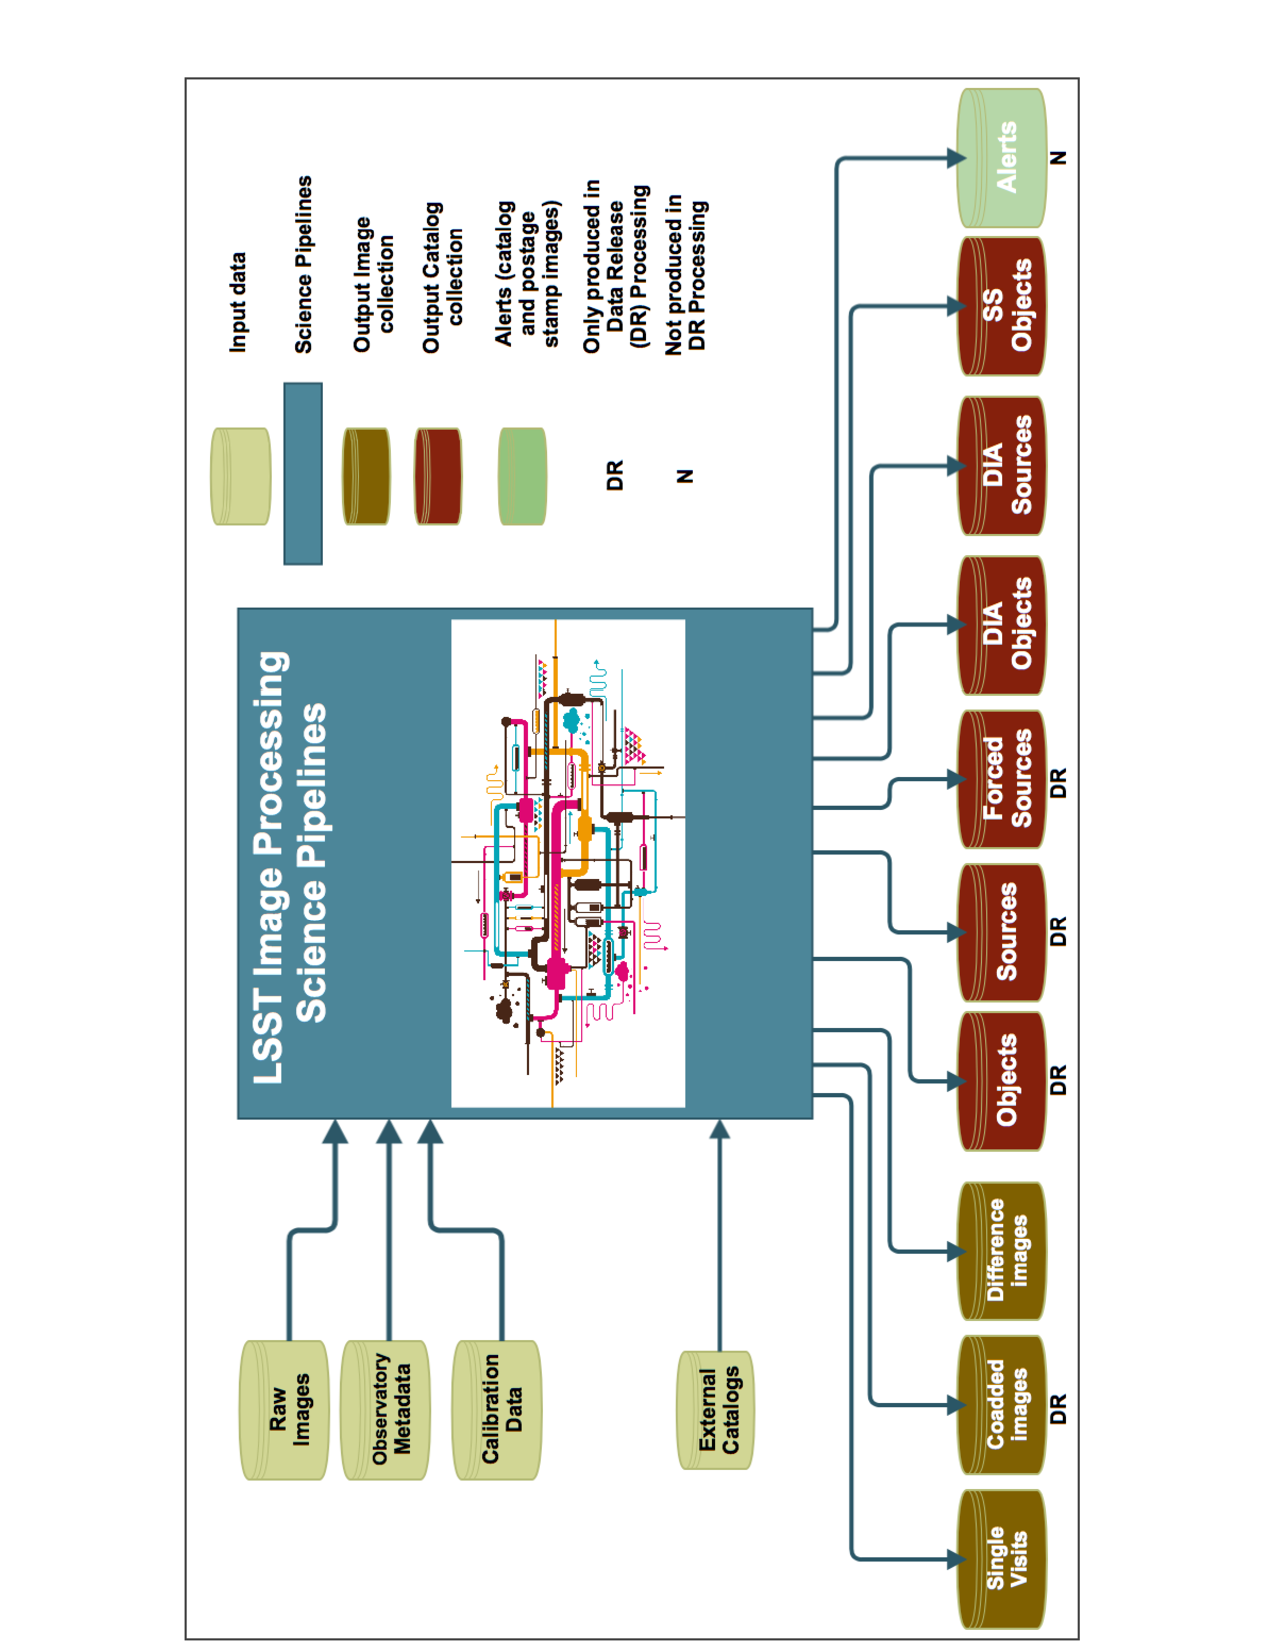
\includegraphics[scale=0.515, angle=270]{gliffy/LSSTimageProcessingDetail0}
    \vskip -0.7in
    \caption{Overview of data products produced by LSST Imaging Processing Science Pipelines.\label{fig:Detail0}}
\end{figure}


\begin{enumerate}
\item Analysis of difference images, with the goal of detecting and characterizing astrophysical phenomena revealed by their time-dependent nature. The detection of supernovae superimposed on bright extended galaxies is an example of this analysis. The processing will be done on nightly or daily basis and result in \textbf{Level 1} data products. Level 1 products will include difference images, catalogs of sources detected in difference images (\DIASources), astrophysical objects\footnote{The LSST has adopted the nomenclature by which single-epoch detections of astrophysical \emph{objects} are called \emph{sources}. The reader is cautioned that this nomenclature is not universal: some surveys call \emph{detections} what LSST calls \emph{sources}, and use the term \emph{sources} for what LSST calls \emph{objects}.} these are associated to (\DIAObjects), and Solar System objects (\SSObjects\footnote{\SSObjects used to be called ``Moving Objects'' in previous versions of the LSST Data Products baseline. The name is potentially confusing as high-proper motion stars are moving objects as well. A more accurate distinction is the one between objects \emph{inside} and \emph{outside} of the Solar System.}). The catalogs will be entered into the \textbf{\DB} and made available in near real time. Notifications (``alerts'') about new \DIASources will be issued using community-accepted
standards\footnote{For example, VOEvent, see \url{http://ls.st/4tt}} within 60 seconds of observation. Level 1 data products are discussed in \S~\ref{sec:level1}.

\item Analysis of direct images, with the goal of detecting and characterizing astrophysical objects. Detection of faint galaxies on deep coadds and their subsequent characterization is an example of this analysis. The results are \textbf{Level 2} data products. These products, generated and released annually\footnote{Except for the first two data releases, which will be created six months apart.}, will include the single-epoch images, deep coadds, catalogs of characterized \Objects (detected on deep coadds as well as individual visits\footnote{The LSST takes two exposures per pointing, nominally 15 seconds in duration each, called \emph{snaps}. For the purpose of data processing, that pair of exposures will typically be coadded and treated as a single exposure, called a \emph{visit}.}), \Sources\footnote{When written in bold monospace type (i.e., \texttt{\textbackslash{}tt}), \Objects and \Sources refer to objects and sources detected and measured as a part of Level 2 processing.} (detections and measurements on individual visits), and \ForcedSources (constrained measurement of flux on individual visits). It will also include fully reprocessed Level 1 data products (see \S \ref{sec:l1dbreproc}). In contrast to the ``living'' \DB, which is updated in real-time, the \DR{}s are static and will not change after release. Level 2 data products are discussed in \S~\ref{sec:level2}.
\end{enumerate}


The two types of analyses have different requirements on timeliness. Changes in flux or position of objects may need to be immediately followed up, lest interesting information be lost. Thus the primary results of analysis of difference images -- discovered and characterized \DIASources{} -- generally need to be broadcast as \emph{event alerts} within 60 seconds\reqparam{OTT1} of end of visit acquisition.\dmreq{0004} The analysis of science (direct) images is less time sensitive, and will be done as a part of annual data release process.

Recognizing the diversity of astronomical community needs, and the need for specialized processing not part of the automatically generated Level 1 and 2 products, LSST plans to devote 10\% of its data management system capabilities to enabling the creation, use, and federation of \textbf{Level 3} (user-created) data products. Level 3 capabilities will enable science cases that greatly benefit from co-location of user processing and/or data within the LSST Archive Center. The high-level requirement for Level 3 is established in \S~3.5 of the LSST \SRD. Their details are discussed in \S~\ref{sec:level3} of this document.

Finally, LSST Survey Specifications (\S~3.4 of LSST \SRD) prescribe that 90\% of LSST observing time be spent in the so-called ``universal cadence'' mode of surveying the sky. These observations will result in Level 1 and 2 data products discussed above. The remaining 10\% of observing time will be devoted to \textbf{special programs}, designed to obtain improved coverage of interesting regions of observational parameter space. Examples include very deep ($r\sim26$, per exposure) observations, observations with very short revisit times ($\sim$1 minute), and observations of ``special'' regions such as the Ecliptic, Galactic plane, and the Large and Small Magellanic Clouds. The data products for these programs will be generated using the same processing software and hardware and possess the general characteristics of Level 1 and 2 data products, but may be performed on a somewhat different cadence. They will be discussed in \S~\ref{sec:specialProgs}.


\section{General Considerations}

Most LSST data products will consist of images and/or catalogs. The catalogs will be stored and offered to the users as \emph{relational databases} which they will be able to query. This approach was shown to work well by prior large surveys, for example the Sloan Digital Sky Survey (SDSS).

Different data products will generally be stored in different databases. For example, Level 1 data products will be stored in a \emph{Level 1 database}. Level 2 ``universal cadence'' products will be stored in a \emph{Level 2 database} database. The products for special programs may be stored in many different databases, depending on the nature of the program.

Nevertheless, all these databases will follow certain naming and other conventions. We discuss these in the subsections to follow.



\subsection{Estimator and Naming Conventions}

For all catalogs data, we will employ a convention where estimates of standard errors have the suffix \texttt{Err}, while the estimates of inherent widths of distribution (or functions in general) have the suffix \texttt{Sigma}\footnote{Given $N$ measurements, standard errors scale as $N^{-1/2}$, while widths remain constant.}. The latter are defined as the square roots of the second moment about the quoted value of the quantity at hand.

\dmreq{0333}
Unless noted otherwise, maximum likelihood values (called likelihood for simplicity) will be quoted for all fitted parameters (measurements). Together with covariances, these let the end-user apply whatever prior they deem appropriate when computing posteriors\footnote{There's a tacit assumption that a Gaussian is a reasonably good description of the likelihood surface around the ML peak.}. Where appropriate, multiple independent samples from the likelihood may be provided to characterize departures from Gaussianity.

We will provide values of log likelihood, the $\chi^2$ for the fitted parameters, and the number of data points used in the fit. \dmreq{0331}Database functions (or precomputed columns) will be provided for frequently used combinations of these quantities (e.g., $\chi^2/dof$). These can be used to assess the model fit quality. Note that, \textit{if the errors of measured quantities are normally distributed,} the likelihood is related to the $\chi^2$ as:
%
\begin{equation}
    L = \left(\prod_{k}\frac{1}{\sigma_k \sqrt{2 \pi}}\right) \exp \left[- \frac{\chi^2}{2}\right]
\end{equation}
%
where the index $k$ runs over all data points included in the fit.
For completeness, $\chi^2$ is defined as:
%
\begin{equation}
      \chi^2 = \sum_{k} \left( \frac{x_k-\bar{x}}{\sigma_k}\right)^2,
\end{equation}
%
where $\bar{x}$ is the mean value of $x_k$.

For fluxes, we recognize that a substantial fraction of astronomers will just want the posteriors marginalized over all other parameters, trusting the LSST experts to select an appropriate prior\footnote{It's likely that most cases will require just the expectation value alone.}. For example, this is nearly always the case when constructing color-color or color-magnitude diagrams. We will support these use cases by \dmreq{0331}providing additional pre-computed columns, taking care to name them appropriately so as to minimize accidental incorrect usage. For example, a column named \texttt{gFlux} may be the expectation value of the g-band flux, while \texttt{gFluxML} may represent the maximum likelihood value.

\subsection{Image Characterization Data}

Raw images will be processed to \dmreq{0069}remove instrumental signature and characterize their properties, \dmreq{0327}including backgrounds (both due to night sky and astrophysical), \dmreq{0070}the point spread function and its variation, \dmreq{0029}photometric zero-point model, and the \dmreq{0030}world coordinate system (WCS).

That characterization is crucial for deriving LSST catalogs and understanding the images. It will be kept and made available to the users. The exact format used to store these (meta)data will depend on the final adopted algorithm in consultation with the scientific community to ensure the formats in which these data are served are maximally useful.\dmreq{0328}

\dmreq{0072}Each processed image\footnote{It is also frequently referred to as \emph{calibrated exposure}, from the Butler product type of \texttt{calexp}.}, including the coadds, will record information on pixel variance (the ``variance plane''), as well as per-pixel masks (the ``mask plane''). These will allow the users to determine the validity and usefullness of each pixel in estimating the flux density recorded in that area of the sky.

This information will be per-pixel, and potentially unwieldy to use for certain science cases. We plan to investigate approximate schemes for storing masks based on geometry (e.g., similar to Mangle or STOMP), \emph{in addition} to storing them on a per pixel basis.\dmreq{0326}

\subsection{Fluxes and Magnitudes}
\label{sec:fluxes}
\dmreq{0043}
Because flux measurements on difference images (Level 1 data products; \S~\ref{sec:level1}) are performed against a template
and thus represent a flux difference, the measured flux of a source on the difference image can be negative. The flux can also go negative for faint sources in the presence of noise. Negative fluxes cannot be stored as (Pogson) magnitudes; $\log$ of a negative number is undefined. We therefore prefer to store fluxes, rather than magnitudes, in database tables\footnote{This is a good idea in general. E.g., given multi-epoch observations, one should always be averaging fluxes, rather than magnitudes.}.\dmreq{0347}

We quote fluxes in units of ``maggie''. A maggie, as introduced by SDSS, is a linear measure of flux. It is defined so that an object having a flux of one maggie (integrated over the bandpass) has an AB magnitude of zero:
\begin{equation}
    m_{AB} = -2.5 \log_{10}(f/\mathrm{maggie})
\end{equation}

We chose to use maggies (as opposed to, say, Jansky) to allow the user to differentiate between two distinct sources of photometric calibration error: the error in relative (internal) calibration of the survey, and the error in absolute calibration that depends on the knowledge of absolute flux of photometric standards.

Nevertheless, we acknowledge that the large majority of users will want to work with magnitudes. For convenience, we plan to provide columns with (Pogson) magnitudes\footnote{These will most likely be implemented as ``virtual'' or ``computed'' columns}, where values with negative flux will evaluate to \code{NULL}. Similarly, we will provide columns with flux expressed in Jy (and its error estimate that includes the relative and absolute calibration error contributions).

\subsection{Uniqueness of IDs across database versions}

\dmreq{0292}
To reduce the likelihood for confusion, all IDs shall be unique across databases and database versions, other than those corresponding to uniquely identifiable entities (i.e., IDs of exposures).

For example, DR4 and DR5 (or any other) release will share no identical \Object, \Source, \DIAObject or \DIASource IDs (see \S~\ref{sec:level1}~and~\ref{sec:level2} for the definitions of \Objects, \DIAObjects, etc.).

\subsection{Repeatability of Queries}
\dmreq{0291}

We require that queries executed at a known point in time against any LSST-delivered database be repeatable at a later date. This promotes the reproducibility of science derived from LSST data. It is of special importance for Level 1 catalogs (\S~\ref{sec:level1}) that will change on a nightly basis as new time domain data is being processed and added to the catalogs.

The exact implementation of this requirement is left to the LSST Data Management database team. One possibility may be to make the key tables (nearly) append-only, with each row having two timestamps -- \texttt{createdTai} and \texttt{deletedTai}, so that queries may be limited by a \code{WHERE} clause:
%
\begin{quote}
\begin{lstlisting}[language=SQL]
SELECT * FROM DIASource WHERE 'YYYY-MM-DD-HH-mm-SS'
    BETWEEN createdTAI and deletedTAI
\end{lstlisting}
\end{quote}
%
or, more generally:
%
\begin{quote}
\begin{lstlisting}[language=SQL,showstringspaces=false]
SELECT * FROM DIASource WHERE "data is valid as of YYYY-MM-DD"
\end{lstlisting}
\end{quote}
%
A perhaps less error-prone alternative, if technically feasible, may be to provide multiple virtual databases that the user would access as:
%
\begin{quote}
\begin{lstlisting}[language=SQL]
CONNECT lsst-dr5-yyyy-mm-dd
SELECT * FROM DIASource
\end{lstlisting}
\end{quote}
%
The latter method would probably be limited to nightly granularity, unless there's a mechanism to create virtual databases/views on-demand.

\clearpage

\section{Level 1 Data Products}
\label{sec:level1}

\subsection{Overview}

Level 1 data products are a result of difference image analysis (DIA; \S \ref{sec:dia}). They include the sources detected in difference images (\DIASources), astrophysical objects that these are associated to (\DIAObjects), identified Solar System objects\footnote{The \SRD considers Solar System object orbit catalog to be a Level 2 data product (LSST \SRD, Sec 3.5). Nevertheless, to successfully differentiate between apparitions of known Solar System objects and other types \DIASources we consider it functionally a part of Level 1.} (\SSObject), and related, broadly defined, metadata (including eg., cut-outs\footnote{Small, $30 \times 30$, sub-images at the position of a detected source. Also known as \emph{postage stamps.}}).

\DIASources are sources detected on difference images (those with the signal-to-noise ratio $S/N>transSNR$ after correlation with the PSF profile, with $transSNR$\reqparam{transSNR} defined in the \SRD and presently set to \transSNR). They represent changes in flux with respect to a deep template. Detections with high probability of being instrumental non-astrophysical artifacts may be excluded. Physically, a \DIASource may be an observation of new astrophysical object that was not present at that position in the template image (for example, an asteroid), or an observation of flux change in an existing source (for example, a variable star). Their flux can be negative (eg., if a source present in the template image reduced its brightness, or moved away). Their shape can be complex (eg., trailed, for a source with proper motion approaching $\sim$deg/day, or ``dipole-like'', if an object's observed position exhibits an offset -- true or apparent -- compared to its position on the template).
Some \DIASources will be caused by background fluctuations; with $transSNR = \transSNR$,
we expect about one such false positive per CCD (of the order 200,000 per typical night). The expected number of false
positives due to background fluctuations is a very strong function of adopted $transSNR$: a change of $transSNR$ by 0.5
results in a variation of an order of magnitude, and a change of $transSNR$ by unity changes the number of false
positives by about two orders of magnitude.

Clusters of \DIASources detected on visits taken at different times are associated with either a \DIAObject or an \SSObject,\dmreq{0285} to represent the underlying astrophysical phenomenon. The association can be made in two different ways: by assuming the underlying phenomenon is an object within the Solar System moving on an orbit around the Sun\footnote{We don't plan to fit for motion around other Solar System bodies; eg., identifying new satellites of Jupiter is left to the community.}, or by assuming it to be distant enough to only exhibit small parallactic and proper motion\footnote{Where 'small' is small enough to unambiguously positionally associate together individual apparitions of the object.}. The latter type of association is performed during difference image analysis right after the image has been acquired. \dmreq{0089}The former is done at daytime by the Moving Objects Processing Software (\code{MOPS}), unless the \DIASource is an apparition of an already known \SSObject. In that case, it will be flagged as such during difference image analysis.

\dmreq{0002}
At the end of the difference image analysis of each visit, we will issue time domain event alerts for all newly %discovered
detected \DIASources\footnote{For observations on the Ecliptic near the opposition Solar System objects will dominate the \DIASource counts and (until they're recognized as such) overwhelm the explosive transient signal. It will therefore be advantageous to quickly identify the majority of Solar System objects early in the survey.}.

\subsection{Level 1 Data Processing}

\subsubsection{Difference Image Analysis}
\label{sec:dia}

The following is a high-level description of steps which will occur during regular \emph{nightly}
difference image analysis (see Figures~\ref{fig:Pipe1} and \ref{fig:Pipes567}):
\begin{enumerate}
\item A visit is acquired and reduced to a single \emph{Processed Visit Image} (cosmic ray rejection, instrumental signature removal\footnote{Eg., subtraction of bias and dark frames, flat fielding, bad pixel/column interpolation, etc.}, combining of snaps, etc.).\dmreq{0069}
\item The Processed Visit Image is differenced against the appropriate template and \DIASources are detected. If necessary, deblending will be performed at this stage. Both the parent blend and the deblended children will be measured and stored as \DIASources (see next item), but only the children will be matched against \DIAObjects and alerted on. Deblended objects will be flagged as such.\dmreq{0010}
\item The flux and shape\footnote{The ``shape'' in this context consists of weighted 2$^\mathrm{nd}$ moments, as well as fits to a trailed source model and a dipole model.} of the DIASource are measured on the difference image. PSF photometry is performed on the Processed Visit Image at the position of the \DIASource to obtain a measure of the total flux.\dmreq{0269}
\item The \DB (see \S \ref{sec:level1db}) is searched for a \DIAObject or an \SSObject with which to positionally associate the newly discovered \DIASource\footnote{The association algorithm will guarantee that a \DIASource is associated with not more than one existing \DIAObject or \SSObject. The algorithm will take into account the parallax and proper (or Keplerian) motions, as well as the errors in estimated positions of \DIAObject, \SSObject, and \DIASource, to find the maximally likely match. Multiple \DIASources in the same visit will not be matched to the same \DIAObject.}. If no match is found, a new \DIAObject is created and the observed \DIASource is associated to it.\dmreq{0273}\dmreq{0271}\dmreq{0285}
\item If the \DIASource has been associated with an \SSObject (a known Solar System object), it will be flagged as such and an alert will be issued. Further processing will occur in daytime (see section \ref{sec:ssProcessing}).\dmreq{0274}
\item Otherwise, the associated \DIAObject measurements will be updated with new data
collected during previous 12 months. Hence, the computed parameters for \DIAObjects have a ``memory'' of past data that does not extend beyond this cutoff\footnote{This restriction is removed when Level 1 processing is
rerun during Data Release production, see \S~\ref{sec:l1dbreproc}.}. All affected columns will be recomputed, including proper motions, centroids, light curves, etc.\dmreq{0319}\reqparam{diaCharacterizationCutoff}
\item The \DR\footnote{\DR is a database resulting from annual data release processing. See \S~\ref{sec:level2} for details.} is searched for the three nearest stars and three nearest galaxies to the \DIAObject in \Objects\reqparam{diaNearbyObjMaxStar}\reqparam{diaNearbyObjMaxGalaxy} out to some maximum radius.\reqparam{diaNearbyObjRadius} The IDs of these nearest-neighbor \Objects are recorded in the \DIAObject record and provided in the issued
event alert (see below).\dmreq{0271}\dmreq{0002}
\item An alert is issued that includes: the name of the \DB, the timestamp of when this database has been queried to issue this alert, the \DIASource ID, the \SSObject ID or \DIAObject ID\footnote{We guarantee that a receiver will always be able to regenerate the alert contents at any later date using the included timestamps and metadata (IDs and database names).}, name of the \DR and the IDs of nearby \Objects, and the associated science content (centroid, fluxes, low-order lightcurve moments, periods, etc.), \emph{including all} \DIASources from the last 12 months\reqparam{diaCharacterizationCutoff} that are linked with the \SSObject or \DIAObject. The science content associated with the \DR \Objects will not be included. See Section \ref{sec:voEventContents} for a more complete enumeration.
\dmreq{0274}
\item For all \DIAObjects overlapping the field of view, including those that have an associated
new \DIASource from this visit, forced photometry will be performed on difference image (point source photometry only). Those measurements will be stored as appropriately flagged \DIASources\footnote{For the purposes of this document, we're treating the \DIASources generated by forced photometry or precovery measurements to be the same as \DIASources detected in difference images (but flagged appropriately). In the logical schema, these may be divided into two separate tables.}.  No alerts will be issued for these \DIASources.\dmreq{0317}
\item Within 24 hours of discovery\reqparam{L1PublicT}, \emph{precovery} PSF forced photometry will be performed on any difference image overlapping the position of new \DIAObjects taken within the past 30 days\reqparam{precoveryWindow}, and added to the database. Alerts will not be issued with precovery photometry information.\dmreq{0287}
\end{enumerate}

In addition to the processing described above, a smaller sample of sources detected on difference images \emph{below} the nominal $transSNR = \transSNR$ \reqparam{transSNR} threshold will be measured and stored, in order to enable monitoring of difference image analysis quality.\dmreq{0270}

Also, the system will have the ability to measure and alert on a limited\footnote{It will be sized for no less than $\sim$10\% of average \DIASource per visit rate.} number of sources detected below the nominal threshold for which additional criteria are satisfied. For example, a $transSNR$ = 3 source detection near a gravitational keyhole\footnote{
A gravitational keyhole is a region of space where Earth's gravity would modify the orbit of a passing asteroid
such that the asteroid would collide with the Earth in the future.}
may be highly significant in assessing the danger posed by a potentially hazardous asteroid.
The initial set of criteria will be defined by the start of LSST operations.

\subsubsection{Solar System Object Processing}
\label{sec:ssProcessing}

The following will occur during regular Solar System object processing (in daytime\footnote{Note that there \emph{is no strict bound on when daytime Solar System processing must finish}, just that, averaged over some reasonable timescale (eg., a month), a night's worth of observing is processed within 24 hours. Nights rich in moving objects may take longer to process, while nights with less will finish more quickly. In other words, the requirement is on \emph{throughput}, not latency.}, after a night of observing; see Figure~\ref{fig:Pipe8}) \dmreq{0004}\dmreq{0089}:
\begin{enumerate}
\item The orbits and physical properties of all \SSObjects re-observed on the previous night are recomputed. External orbit catalogs (or observations) are also used to improve orbit estimates.\dmreq{0288} Updated data are entered to the \SSObjects table.\dmreq{0273}
\item All \DIASources detected on the previous night, that have \emph{not} been matched at a high confidence level to a known \Object,
\DIAObject, \SSObject, or an artifact, are analyzed for potential pairs, forming \emph{tracklets}.
\item The collection of tracklets collected over the past 30 days\footnote{The exact time period is a design and computational question discussed in \citeds{LDM-156}.} is searched for subsets forming \emph{tracks} consistent with being on the same Keplerian orbit around the Sun.
\item For those that are, an orbit is fitted and a new \SSObject table entry created. \DIASource records are updated to point to the new \SSObject record. \DIAObjects ``orphaned'' by this unlinking are deleted.\footnote{Some \DIAObjects may only be left with forced photometry measurements at their location (since all \DIAObjects are force-photometered on previous and subsequent visits);  these will be kept but flagged as such.}.
\item Precovery linking is attempted for all \SSObjects whose orbits were updated in this process.\dmreq{0286} Where successful, \SSObjects (orbits) are recomputed as needed.
\end{enumerate}

\subsection{Level 1 Catalogs}
\label{sec:level1db}

The described alert processing design relies on the ``living'' \DB that contains the objects and sources detected on difference images. At the very least\footnote{It will also contain exposure and visit metadata, MOPS-specific tables, etc. These are either standard/uncontroversial, implementation-dependent, or less directly relevant for science and therefore not discussed in this document.}, this database will have tables of \DIASources,\dmreq{0269} \DIAObjects,\dmreq{0271} and \SSObjects,\dmreq{0273} populated in the course of nightly and daily difference image and Solar System object processing\footnote{The latter is also colloquially known as \emph{DayMOPS}.}. As these get updated and added to, their updated contents becomes visible (query-able) immediately\footnote{No later than the moment of issuance of any event alert that may refer to it.}.\dmreq{0312}

This database is \emph{only loosely coupled to the \DR}. All of the coupling is through positional matches between the \DIAObjects entries in the \DB and the \Objects in the \DR database. There is no direct \DIASource-to-\Object match:
in general, a time-domain object is not necessarily the same astrophysical object as a static-sky object, even if the two are
positionally coincident (eg. an asteroid overlapping a galaxy).
Therefore, adopted data model emphasizes that \emph{having a \DIASource be positionally coincident with an \Object does not imply it is physically related to it}. Absent other information, the least presumptuous data model relationship is one of \emph{positional association}, not \emph{physical identity}.

This may seem odd at first: for example, in a simple case of a variable star, matching individual \DIASources to \Objects is exactly what an astronomer would want. That approach, however, fails in the following scenarios:
\begin{itemize}
    \item \emph{A supernova in a galaxy.} The matched object in the \Object table will be the galaxy, which is a distinct astrophysical object. We want to keep the information related to the supernova (eg., colors, the light curve) separate from those measurements for the galaxy.
    \item \emph{An asteroid occulting a star.} If associated with the star on first apparition, the association would need to be dissolved when the source is recognized as an asteroid (perhaps even as early as a day later).
    \item \emph{A supernova on top of a pair of blended galaxies.} It is not clear in general to which galaxy this \DIASource would ``belong''. That in itself is a research question.
\end{itemize}

\DIASource-to-\Object matches can still be emulated via a two-step relation (\DIASource-\DIAObject-\Object). For ease of use, views or pre-built table with these matches will be offered to the end-users.\dmreq{0324}

% There are three ``core'' tables in the \DB: the \DIASource table, with information about detected and/or measured \DIASources, \DIAObject table, with summary information about \DIAObjects derived from the associated \DIASources, and the \SSObject table (short for \textbf{Solar System Object}\footnote{This is what we used to call a ``Moving Object''. This name is potentially confusing, as high-proper motion stars are moving objects as well. A more accurate distinction is the one between objects in an out of the Solar System.}) holding derived orbits and associated Solar System Object-specific information.

In the sections to follow, we present the \emph{conceptual schemas} for the most important \DB tables. These convey \emph{what} data will be recorded in each table, rather than the details of \emph{how}. For example, columns whose type is an array (eg., \texttt{radec}) may be expanded to one table column per element of the array (eg., \texttt{ra}, \texttt{decl}) once this schema is translated to SQL\footnote{The SQL realization of this schema is defined in the \texttt{cat} package and documented in \citeds{LDM-153} and can be browsed at \url{http://ls.st/8g4}}. Secondly, the tables to be presented are largely normalized (i.e., contain no redundant information). For example, since the band of observation can be found by joining a \DIASource table to the table with exposure metadata, there's no column named \texttt{band} in the \DIASource table. In the as-built database, the views presented to the users will be appropriately denormalized for ease of use.

\subsubsection{\DIASource Table}

This is a table of sources detected at $transSNR \geq \transSNR$ \reqparam{transSNR} on difference images\footnote{This requirement is specified in the LSST \SRD.}\lsrreq{0101} (\DIASources).
On average, the LSST \SRD expects
up to
$\sim$10,000 astrophysical \DIASources per visit ($\sim$10M per night; 100,000 per deg$^2$
of the sky per hour).
\reqparam{transN}

Some $transSNR \geq \transSNR$ sources will not be caused by observed astrophysical phenomena, but by artifacts (bad columns, diffraction spikes, etc.). The difference image analysis software will attempt to identify and flag these as such.

Unless noted otherwise, all \DIASource quantities (fluxes, centroids, etc.) are measured on the difference image.

\dmreq{0269}

\begin{schema}{\DIASource Table}{\DIASource Table}{tbl:diasourceTable}

diaSourceId & uint64 & ~ & Unique source identifier \\

ccdVisitId & uint64 & ~ & ID of CCD and visit where this source was measured \\

diaObjectId & uint64 & ~ & ID of the \DIAObject this source was associated with, if any. \\

ssObjectId & uint64 & ~ & ID of the \SSObject this source has been linked to, if any. \\

parentDiaSourceId & uint64 & ~ & ID of the parent \DIASource this object has been deblended from, if any. \\

midPointTai & double & time & Time of mid-exposure for this DIASource\footnote{The visit mid-exposure
time generally depends on the position of the source relative to the shutter blade motion trajectory.}. \\

radec & double[2] & degrees & Centroid, $(\alpha, \delta)$\footnote{The astrometric reference frame will be chosen closer to start of operations.}. \\

radecCov & float[3] & various & \texttt{radec} covariance matrix. \\

xy & float[2] & pixels & Column and row of the centroid. \\

xyCov & float[3] & various & Centroid covariance matrix. \\

apFlux & float & nmgy & Calibrated aperture flux. Note that this actually measures
the flux \emph{difference} between the template and the visit image. \\

apFluxErr & float & nmgy &  Estimated uncertainty of \texttt{apFlux}. \\

SNR & float & ~ & The signal-to-noise ratio at which this source was detected in the difference image.\footnote{This is not necessarily the same as apFlux/apFluxErr, as the flux measurement algorithm may be more accurate than the detection algorithm.} \\

psFlux & float & nmgy\footnote{A ``maggie'', as introduced by SDSS, is a linear measure of flux in units of 3631 Jy; one maggie has an AB magnitude of 0, $m_{AB}=-2.5\log_{10}(\mathrm{maggie})$. ``nmgy'' is short for a nanomaggie (1 nmgy = 3.631 $\mu Jy$). For example, a flux of $0.158$~nmgy corresponds to AB magnitude of $24.5$. See \S \ref{sec:fluxes} for details.} & Calibrated flux for point source model. Note this actually measures the flux \emph{difference} between the template and the visit image. \\

psRadec & double[2] & degrees & Centroid for point source model. \\

psCov & float[6] & various & Covariance matrix for point source model parameters. \\

psLnL & float & ~ & Natural $log$ likelihood of the observed data given the point source model. \\

psChi2 & float & ~ & $\chi^2$ statistic of the model fit. \\

psNdata & int & ~ & The number of data points (pixels) used to fit the model. \\

trailFlux & float & nmgy & Calibrated flux for a trailed source model\footnote{A \emph{Trailed Source Model} attempts to fit a (PSF-convolved) model of a point source that was trailed by a certain amount in some direction (taking into account the two-snap nature of the visit, which may lead to a dip in flux around the mid-point of the trail). Roughly, it's a fit to a PSF-convolved line. The primary use case is to characterize fast-moving Solar System objects.}$^,$\footnote{This model does not fit for the \emph{direction} of motion; to recover it, we would need to fit the model to separately to individual snaps of a visit. This adds to system complexity, and is not clearly justified by increased MOPS performance given the added information.}. Note this actually measures the flux \emph{difference} between the template and the visit image. \\

trailRadec & double[2] & degrees & Centroid for trailed source model. \\

trailLength & float & arcsec & Maximum likelihood fit of trail length\footnote{Note that we'll likely measure trailRow and trailCol, and transform to trailLength/trailAngle (or trailRa/trailDec) for storage in the database. A stretch goal is to retain both.}$^,$\footnote{TBD: Do we need a separate trailCentroid? It's unlikely that we do, but one may wish to prove it.}. \\

trailAngle & float & degrees & Maximum likelihood fit of the angle between the meridian through the centroid and the trail direction (bearing, direction of motion). \\

trailCov & float[15] & various & Covariance matrix of trailed source model parameters. \\

trailLnL & float & ~ & Natural $log$ likelihood of the observed data given the trailed source model. \\

trailChi2 & float & ~ & $\chi^2$ statistic of the model fit. \\

trailNdata & int & ~ & The number of data points (pixels) used to fit the model. \\

dipMeanFlux & float & nmgy & Maximum likelihood value for the mean absolute flux of the two lobes for a dipole model\footnote{A \emph{Dipole Model} attempts to fit a (PSF-convolved) model of two point sources, with fluxes
of opposite signs, separated by a certain amount in some direction. The primary use case is to characterize moving stars and problems with image differencing (e.g., due to astrometric offsets).}.
\\

dipFluxDiff & float & nmgy & Maximum likelihood value for the difference of absolute fluxes of the two lobes for a dipole model.
\\

dipRadec & double[2] & degrees & Centroid for dipole model. \\

dipLength & float & arcsec & Maximum likelihood value for the lobe separation in dipole model. \\

dipAngle & float & degrees & Maximum likelihood fit of the angle between the meridian through the centroid and the dipole direction (bearing, from negative to positive lobe). \\

dipCov & float[21] & various & Covariance matrix of dipole model parameters. \\

dipLnL & float & ~ & Natural $log$ likelihood of the observed data given the dipole source model. \\

dipChi2 & float & ~ & $\chi^2$ statistic of the model fit. \\

dipNdata & int & ~ & The number of data points (pixels) used to fit the model. \\

totFlux & float & nmgy & Calibrated flux for point source model measured on the visit image centered at the centroid measured on the difference image (forced photometry flux) \\

totFluxErr & float & nmgy & Estimated uncertainty of \texttt{fpFlux}. \\

diffFlux & float & nmgy & Calibrated flux for point source model centered on \texttt{radec} but measured on the difference of snaps comprising this visit\footnote{This flux can be used to detect sources changing on timescales comparable to snap exposure length ($\sim$15\,sec).}. \\

diffFluxErr & float & nmgy & Estimated uncertainty of \texttt{diffFlux}. \\

fpBkgd & float & nmgy/asec$^{2}$ & Estimated background at the position (centroid) of the object in
the template image. \\

fpBkgdErr & float & nmgy/asec$^{2}$ & Estimated uncertainty of \texttt{fpBkgd}. \\

%grayExtinction & float & nmgy & Applied photometric extinction correction (gray component) \\

%nonGrayExtinction & float & nmgy & Applied photometric extinction correction (color-dependent component) \\

Ixx & float & asec$^{2}$  & Adaptive second moment of the source intensity. See \citet{2002AJ....123..583B} for detailed discussion of all adaptive-moment related quantities\footnote{Or \url{http://ls.st/5f4} for a brief summary.}. \\

Iyy & float & asec$^{2}$ & Adaptive second moment of the source intensity. \\

Ixy & float & asec$^{2}$ & Adaptive second moment of the source intensity. \\

Icov & float[6] & asec$^{4}$ & \texttt{Ixx}, \texttt{Iyy}, \texttt{Ixy} covariance matrix. \\

IxxPSF & float & asec$^{2}$ & Adaptive second moment for the PSF. \\

IyyPSF & float & asec$^{2}$ & Adaptive second moment for the PSF. \\

IxyPSF & float & asec$^{2}$ & Adaptive second moment for the PSF. \\

extendedness & float & ~ & A measure of extendedness, computed using a combination of available moments, or from a likelihood ratio of point/trailed source models (exact algorithm TBD). $extendedness=1$ implies a high degree of confidence that the source is extended. $extendedness=0$ implies a high degree of confidence that the source is point-like. \\

spuriousness & float & ~ & A measure of spuriousness, computed using information\footnote{The computation
of spuriousness will be “prior free” to the extent possible and not use any information about the astrophysical neighborhood of the source, whether it has been previously observed or not, etc. The intent is to avoid introducing
a bias against unusual sources or sources discovered in unusual environments.}
from the source and image characterization, as well as the information on the Telescope and Camera system
(e.g., ghost maps, defect maps, etc.).
\\

flags & bit[64] & bit & Various useful flags.  \\
\end{schema}

Some fast-moving, trailed, sources may be due to passages of nearby asteroids. Their trails may exhibit significant curvature.
While we do not measure the curvature directly, it can be inferred by examining the length of the trail, the trailed model covariance matrices, and the adaptive shape measures. Once curvature is suspected, the users may fit curved trail models to the cutout provided with the alert.

\begin{changelog}
Notes about changes with respect to the previous baseline:
\begin{itemize}
    \item I removed the \texttt{astromRefr*} columns. These will depend on the SED (color) of the object, and the color won't be know when the object is discovered. It may be better to provide a UDF to compute the refraction given a \DIAObject record.
    \item Removed ``small galaxy'' model fits. We don't plan to do galaxy model fits on difference images.
    \item Removed ``canonical small galaxy'' model fits. See above.
    \item Removed galExtinction: this should be a UDF using extinction maps
    \item I removed the aperture correction column.
    \item gray/nonGray extinction columns removed. May be implemented as an UDF.
    \item TODO: See what other fields SDSS has. Also see what fields PanSTARRS has. Collect input from SCs.
\end{itemize}
\end{changelog}

\subsubsection{\DIAObject Table}

\dmreq{0271}\dmreq{0272}\reqparam{diaNearbyMaxObj}

\begin{schema}{\DIAObject Table}{\DIAObject Table}{tbl:diaobjectTable}

diaObjectId & uint64 & ~ & Unique identifier. \\

radec & double[2] & degrees & $(\alpha, \delta)$ position of the object at time \texttt{radecTai}. \\

radecCov & float[3] & various & \texttt{radec} covariance matrix. \\

radecTai & double & time & Time at which the object was at a position \texttt{radec}. \\

pm & float[2] & mas/yr & Proper motion vector\footnote{High proper-motion or parallax objects will appear as ``dipoles'' in difference images. Great care will have to be taken not to misidentify these as subtraction artifacts.}. \\

parallax & float & mas & Trigonometric arallax. \\

pmParallaxCov & float[6] & various & Proper motion - parallax covariances. \\

pmParallaxLnL & float & ~ & Natural log of the likelihood of the linear proper motion-parallax fit\footnote{\texttt{radec}, \texttt{pm}, and \texttt{parallax} will all be simultaneously fitted for.}. \\

pmParallaxChi2 & float & ~ & $\chi^2$ statistic of the model fit. \\

pmParallaxNdata & int & ~ & The number of data points used to fit the model. \\

psFluxMean & float[ugrizy] & nmgy & Weighted mean of point-source model flux, \texttt{psFlux}. \\

psFluxMeanErr & float[ugrizy] & nmgy & Standard error of \texttt{psFluxMean}.  \\

psFluxSigma & float[ugrizy] & nmgy & Standard deviation of the distribution of \texttt{psFlux}. \\

psFluxChi2 & float[ugrizy] & ~ & $\chi^2$ statistic for the scatter of \texttt{psFlux} around \texttt{psFluxMean}. \\

psFluxNdata & int[ugrizy] & ~ & The number of data points used to compute \texttt{psFluxChi2}. \\

fpFluxMean & float[ugrizy] & nmgy & Weighted mean of forced photometry flux, \texttt{fpFlux}.\\

fpFluxMeanErr & float[ugrizy] & nmgy & Standard error of \texttt{fpFluxMean}. \\

fpFluxSigma & float[ugrizy] & nmgy & Standard deviation of the distribution of \texttt{fpFlux}. \\

% lsPeriod  & float[ugrizy] & day & Period (the coordinate of the highest peak in Lomb-Scargle periodogram) \\

% lsSigma  & float[ugrizy] & day & Width of the peak at \texttt{lsPeriod}. \\

% lsPower   & float[ugrizy] & ~ & Power associated with \texttt{lsPeriod} peak. \\

% lcChar   & float[$6\times{}M$] & ~ & Light-curve characterization summary statistics (eg., 2nd moments, etc.). The exact contents, and an appropriate value of M, are to be determined in consultation with time-domain experts. \\

lcPeriodic & float[6~\x~32] & ~ & Periodic features extracted from light-curves using generalized Lomb-Scargle periodogram \citep[Table~4,][]{2011ApJ...733...10R}\footnote{The exact features in use when LSST begins operations are likely to be different compared to the baseline described here. This is to be expected given the rapid pace of research in time domain astronomy. However, the \emph{number} of computed features is unlikely to grow beyond the present estimate.}. \\

lcNonPeriodic & float[6~\x~20] & ~ & Non-periodic features extracted from light-curves \citep[Table~5,][]{2011ApJ...733...10R}. \\

nearbyObj   & uint64[6] & ~ & Closest \Objects\ (3 stars and 3 galaxies) in \DR.\\

nearbyObjDist   & float[6] & arcsec & Distances to \texttt{nearbyObj}. \\

nearbyObjLnP   & float[6] & ~ &  Natural $\log$ of the probability that the observed \DIAObject is the same as the nearby \Object\footnote{This quantity will be computed by marginalizing over the product of position and proper motion error ellipses of the \Object and \DIAObject, assuming an appropriate prior.}. \\

flags & bit[64] & bit & Various useful flags. \\

\end{schema}

\subsubsection{\SSObject Table}

\dmreq{0273}

\begin{schema}{\SSObject Table}{\SSObject Table}{tbl:ssobjectTable}

ssObjectId & uint64 & ~ & Unique identifier. \\

oe & double[7] & various & Osculating orbital elements at epoch ($q$, $e$, $i$, $\Omega$, $\omega$, $M_0$, epoch). \\

oeCov & double[28] & various & Covariance matrix for \texttt{oe}. \\

arc & float & days & Arc of observation. \\

orbFitLnL & float & ~ & Natural log of the likelihood of the orbital elements fit. \\

orbFitChi2 & float & ~ & $\chi^2$ statistic of the orbital elements fit. \\

orbFitNdata & int & ~ & The number of data points (observations) used to fit the orbital elements. \\

MOID & float[2] & AU & Minimum orbit intersection distances\footnote{\url{http://www2.lowell.edu/users/elgb/moid.html}} \\

moidLon & double[2] & degrees & MOID longitudes. \\

H & float[6] & mag & Mean absolute magnitude, per band \citep[][magnitude-phase system]{2010Icar..209..542M}. \\

$\mathrm{G_1}$ & float[6] & mag & $G_1$ slope parameter, per band \citep[][magnitude-phase system]{2010Icar..209..542M}. \\

$\mathrm{G_2}$ & float[6] & mag & $G_2$ slope parameter, per band \citep[][magnitude-phase system]{2010Icar..209..542M}. \\

hErr & float[6] & mag & Uncertainty of H estimate.\\

g1Err & float[6] & mag & Uncertainty of $G_1$ estimate. \\

g2Err & float[6] & mag & Uncertainty of $G_2$ estimate. \\

flags & bit[64] & bit & Various useful flags. \\

\end{schema}

The $G_1$ and $G_2$ parameters for the large majority of asteroids will not be well constrained until later in the survey. We may decide not to fit for it at all over the first few DRs and add it later in Operations, or provide two-parameter $G_{12}$ fits. Alternatively, we may fit it using strong priors on slopes poorly constrained by the data. The design of the data management system is insensitive to this decision, making it possible to postpone it to Commissioning to ensure it follows the standard community practice at that time.

The LSST database will provide functions to compute the phase (Sun-Asteroid-Earth) angle $\alpha$ for every observation, as well as the reduced, $H(\alpha)$, and absolute, $H$, asteroid magnitudes in LSST bands.\dmreq{0323}

\begin{changelog}
Notes about changes with respect to the previous baseline:
\begin{itemize}
    \item Though many columns have been removed, we should maintain roughly the equivalent extra columns in the sizing model as some may re-appear internally (eg., MOPS-specific columns). This is true in general for all tables.
    \item Removed all asteroid shape-related columns; determining these is outside of the scope of the Project.
    \item Removed taxonomy related columns; determining these is outside of the scope of the Project.
    \item Removed \texttt{albedo} -- I don't believe albedo can be determined solely from LSST data. More likely, we will need to assume a particular value. If this value is not universal, this column will need to be put back in.
    \item Removed \texttt{xMag, xMagErr, xAmplitude, xPeriod} columns as they were not clearly defined (eg., w/o phase correction, do they make sense?). These can be recovered by querying the \DIASource table for magnitudes. Deriving phase-corrected light curves is left as a Level 3 task.
    \item Removed a number of other MOPS-specific columns. These are algorithm-specific and should not be a part of the baseline, outward-facing, schema\footnote{Because we may change the algorithm and they may disappear; the scientists should not be relying on them being there.}. They will need to be documented and added back into the physical schema, for sizing purposes.
\end{itemize}
\end{changelog}

\subsubsection{Precovery Measurements}

When a new \DIASource is detected, it's useful to perform PSF photometry at the location of the new source on images taken prior to discovery. These are colloquially known as \emph{precovery measurements}\footnote{When Solar System objects are concerned, precovery has a slightly different meaning: predicting the positions of newly identified \SSObjects on previously acquired visits, and associating with them the \DIASources consistent with these predictions.}.\dmreq{0287}\dmreq{0286} Performing precovery in real time over all previously acquired visits is too I/O intensive to be feasible. We therefore plan the following:
\begin{enumerate}
\item For all newly discovered objects, perform precovery PSF photometry on visits taken over the previous 30 days\reqparam{precoveryWindow}\footnote{We will be maintaining a cache of $30$ days of processed images to support this feature.}.
\item Make available a ``precovery service'' to request precovery for a limited number of \DIASources across all previous visits, and make it available within 24 hours of the request. Web interface and machine-accessible APIs will be provided.\dmreq{0341}
\end{enumerate}

The former should satisfy the most common use cases (eg., SNe), while the latter will provide an opportunity for more extensive yet timely precovery of targets of special interest.

\subsubsection{Reprocessing the Level 1 Data Set}
\label{sec:l1dbreproc}

In what we've described so far, the ``living'' \DB is continually being added to as new images are taken and \DIASources identified.\dmreq{0312} Every time a new \DIASource is associated to an existing \DIAObject, the \DIAObject record is updated to incorporate new information brought in by the \DIASource. Once discovered and measured, the \DIASources would never be re-discovered and re-measured at the pixel level.

This would be far from optimal. The instrument will be better understood with time. Newer versions of LSST pipelines will improve detection and measurements on older data. Also, precovery photometry should optimally be performed for \emph{all} objects, and not just a select few. This argues for periodic \emph{reprocessing} of the Level 1 data set. \dmreq{0313}\dmreq{0325}

We plan to reprocess all image differencing-derived data (the \DB), at the same time we perform the annual Level 2 data release productions. This will include all images taken since the start of survey operations, to the time when the data release production begins. The images will be reprocessed using a single version of the image differencing and measurement software, resulting in a consistent data set.

There will be three main advantages of \DB produced during Data Release processing, compared to
``living'' \DB:
i) even the oldest data will be processed with the latest software,
ii) astrometric and photometric calibration will be better, and
iii) there will be no 12-month limit on the width of data window used to computed associated \DIAObject
measurements (proper motions, centroids, light curves, etc.). \reqparam{diaCharacterizationCutoff}

Older versions of the \DB\ produced during Data Release processing will be archived following the same rules as for the \DR{}s. The most recent DR, and the penultimate data release will be kept on disk and loaded into the database.\dmreq{0077} Others will be archived to tape and made available as bulk downloads.\dmreq{0300} See \S~\ref{sec:retention} for more detail.

\subsection{Level 1 Image Products}

\subsubsection{Visit Images}
\dmreq{0069}

Raw and Processed Visit Images will be made available for download no later than 24 hours\reqparam{L1PublicT} from the end of visit acquisition.

The images will remain accessible with low-latency (seconds from request to start of download) for at least 30 days\reqparam{l1CacheLifetime}, with slower access afterwards (minutes to hours).

\subsubsection{Difference Images}
\label{sec:diffims}
\dmreq{0010}

Complete difference images will be made available for download no later than 24 hours\reqparam{L1PublicT} from the end of visit acquisition.

The images will remain accessible with low-latency (seconds from request to start of download) for at least 30 days\reqparam{l1CacheLifetime}, with slower access afterwards (minutes to hours).

\subsubsection{Image Differencing Templates}
\label{sec:templates}
\dmreq{0280}

Templates for difference image analysis will be created by coadding 6-months to a year long groups of visits. The coaddition process will take care to remove transient or fast moving objects (eg., asteroids) from the templates.
Difference image analysis will use the appropriate template given the time of observation, airmass, and seeing.

\subsection{Alerts to \DIASources}
\label{sec:voEventContents}

\subsubsection{Information Contained in Each Alert}

For each detected \DIASource, LSST will emit an ``Event Alert'' within 60 seconds\reqparam{OTT1} of the end of visit (defined as the end of image readout from the LSST Camera). These alerts will be issued in \VOEvent format\footnote{Or some other format that is broadly accepted and used by the community at the start of LSST commissioning.}, and should be readable by \VOEvent-compliant clients.\dmreq{0002}

Each alert (a \VOEvent packet) will at least include the following:

\begin{itemize}
    \item \emph{alertID}: An ID uniquely identifying this alert. It can also be used to execute a query against the \DB as it existed when this alert was issued.\dmreq{0274}
    \item \emph{\DB ID}   %: For example, \texttt{DR5L1}
    \item Science Data:
    \begin{itemize}
        \item The \DIASource record that triggered the alert
        \item The entire \DIAObject (or \SSObject) record
        \item Previous 12 months of \DIASource records\reqparam{diaCharacterizationCutoff}
        \item Matching \Object IDs from the latest Data Release, if they exist, and 12 months of their \DIASource records
    \end{itemize}
    % \item Flags (isSolarSystemObject, isArtefact, etc.)
    \item Cut-out of the difference image centered on the \DIASource (10 bytes/pixel, FITS MEF)
    \item Cut-out of the template image centered on the \DIASource (10 bytes/pixel, FITS MEF)
\end{itemize}

The variable-size cutouts will be sized so as to encompass the entire footprint of the detected source, but be no smaller than $30 \times 30$ pixels. The provided images will comprise of a flux (32 bit float), variance (32 bit float), and mask (16 bit flags) planes, and include metadata necessary for further processing (e.g., WCS, zero-point, PSF, etc.).

The items above are meant to represent the \emph{information} transmitted with each alert; the content of the alert packet itself will be formatted to confirm to \VOEvent (or other relevant) standard. Where the existing standard is inadequate for LSST needs, LSST will propose extensions and work with the community to reach a common solution.

With each alert, we attempt to include as much information known to LSST about the \DIASource as possible, to minimize the need for follow-up database queries. This speeds up classification and decision making at the user end, and relaxes the requirements on the database on the Project end.

\subsubsection{Receiving and Filtering the Alerts}
\label{sec:eventbrokers}

Alerts will be transmitted in \VOEvent format, using standard IVOA protocols\dmreq{0002} (e.g., VOEvent Transport Protocol; VTP\footnote{VOEvent Transport Protocol is currently an IVOA Note, but we understand work is under way to finalize and bring it up to full IVOA Recommendation status.}). As a very high rate of alerts is expected, approaching $\sim$10 million per night, we plan for public VOEvent Event Brokers\footnote{These brokers are envisioned to be operated as a public service by third parties who will have signed MOUs with LSST.} to be the primary end-points of LSST's event streams. End-users will use these brokers to classify and filter events for subsets fitting their science goals. End-users will \emph{not} be able to subscribe to full, unfiltered, alert streams coming directly from LSST\footnote{This is due to finite network bandwidth available: for example, 100 end-users subscribing to a $\sim$100\,Mbps stream (the peak full stream data rate at end of the first year of operations) would require 10Gbps WAN connection from the archive center, just to serve the alerts.}.

To directly serve the end-users, LSST will provide a basic, limited capacity, alert filtering service.\dmreq{0342} This service will run at the LSST U.S. Archive Center (at NCSA). It will let astronomers create simple filters that limit what alerts are ultimately forwarded to them\footnote{More specifically, to their VTP clients. Typically, a user will use the Science User Interface (the web portal to LSST Archive Center) to set up the filters, and use their VTP client to receive the filtered \VOEvent stream.}. These \emph{user defined filters} will be possible to specify using an SQL-like declarative language, or short snippets of (likely Python) code. For example, here's what a filter may look like:

\begin{lstlisting}[language=python,commentstyle=\bfseries\color{green!40!black}]
    # Keep only never-before-seen events within two
    # effective radii of a galaxy. This is for illustration
    # only; the exact methods/members/APIs may change.

    def filter(alert):
        if len(alert.sources) > 1:
            return False
        nn = alert.diaobject.nearest_neighbors[0]
        if not nn.flags.GALAXY:
            return False
        return nn.dist < 2. * nn.Re
\end{lstlisting}


We emphasize that this LSST-provided capability will be limited, and is \emph{not} intended to satisfy the wide variety of use cases that a full-fledged public Event Broker could.
For example, we do not plan to provide any \emph{exclusive} classification to a unique category of object.
Following the \SRD specification, however, we will provide a limited number of pre-defined filters for a small number of object types of common interest.\dmreq{0348}
These will answer non-exclusive questions such as ``is the light curve consistent with an RR Lyra?'', and will have potentially highly overlapping selections, designed to provide good completeness but perhaps only very modest purity.
No information beyond what is contained in the \VOEvent packet will be available to the pre-defined or user-defined filters (e.g., no cross-matches to other catalogs).
The complexity and run time of user defined filters will be limited by available resources.
Execution latency will not be guaranteed.
The number of \VOEvents transmitted to each user per visit will be limited as well (e.g., the equivalent of 20 full-size alert packets per visit per user\reqparam{numBrokerAlerts}\dmreq{0343}, dynamically throttled depending on load).
Finally, the total number of simultaneous subscribers is likely to be limited\reqparam{numBrokerUsers} -- in case of overwhelming interest, a TAC-like proposal process may be instituted.

\begin{openissues}
\subsection{Open Issues}

What follows is a (non-exhaustive) list of issues, technical and scientific, that are still being discussed and where changes are possible. The estimate of the time by which a decision should be made is noted in parentheses.

\begin{itemize}
    \item \emph{Should we measure on individual snaps (or their difference)?} Is there a demonstrable science case requiring immediate followup that would be triggered by the flux change over a $\sim$15 second period? Is it technically feasible? (FDR)
    \item \emph{Is \DB required to be relational?}. A no-SQL solution may be more appropriate given the followup-driven use cases. Even if it is relational, the Level 1 database will \emph{not} be sized or architected to perform well on large or complex queries (eg. complex joins, full table scans, etc.). (FDR)
    \item \emph{Should we associate alerts with external catalogs?}. LSST will have a copy of many external catalogs (or parts thereof), and could in principle provide limited positional association. Right now, it's up to the downstream brokers to perform such associations. (CONSTRUCTION)
    \item \emph{Can we, should we, and how will we measure proper motions on difference images?} This is a non-trivial task (need to distinguish between dipoles that are artifacts, and those due to proper motions), without a clear science driver (since high proper motion stars will be discoverable using Level 2 catalogs). (CONSTRUCTION)
    \item \emph{What light-curve metric should we compute and provide with alerts?} We strive to compute general purpose metrics which will facilitate classification. We have currently baselined the \citet{2011ApJ...733...10R} feature set. (COMMISSIONING)
    \item \emph{Should we choose \texttt{nearbyObj}s differently?} One proposal is to find the brightest \Object within $XX$ arcsec (with $XX \sim$10\,arcsec), and the total number of \Objects within $XX$ arcsec. (COMMISSIONING)
    \item \emph{Should the postage stamps provided with the alerts be binned, and by what factor?} The thought is that a human user may have an easier time performing a final by-eye check with larger postage stamps. (COMMISSIONING)
    \item \emph{When should we (if ever) stop performing forced photometry on positions of \DIAObjects?} Depending on the rate of false positives, unidentified artifacts, or unrecognized Solar System objects, the number of forced measurements may dramatically grow over time. (OPERATIONS)

\end{itemize}
\end{openissues}

\clearpage

\section{Level 2 Data Products}
\label{sec:level2}

\subsection{Overview}

Level 2 data products result from direct image\footnote{As opposed to \emph{difference image}, for Level 1.} analysis. They're designed to enable \emph{static sky} science (eg., studies of galaxy evolution, or weak lensing), and time-domain science that is not time sensitive (eg. statistical investigations of variability). They include image products (reduced single-epoch exposures, called \emph{Processed Visit Images} or, sometimes, \emph{calibrated exposures},\dmreq{0069} and coadds\dmreq{0279}\dmreq{0281}), and catalog products (tables of objects\dmreq{0275}, sources\dmreq{0267}, their measured properties\dmreq{0276}, and related metadata).

Similarly to Level 1 catalogs of \DIAObjects and \DIASources, \Objects in the Level 2 catalog\dmreq{0275} represent the astrophysical phenomena (stars, galaxies, quasars, etc.), while \Sources represent their single-epoch observations. \Sources are independently detected and measured in single epoch exposures and recorded in the \Source table.\dmreq{0267}

The master list of \Objects in Level 2 will be generated by associating and deblending the list of single-epoch \DIASource detections and the lists of sources detected on coadds (\CoaddSources).\dmreq{0275} We plan to build coadds designed to maximize depth (\emph{``deep coadds''})\dmreq{0279} and coadds designed to achieve a good combination of depth and seeing (\emph{``best seeing coadds''}), unless
algorithms will enable these two to be the same.\dmreq{0330}
We will also build a series of \emph{short-period} (eg. yearly, or multi-year) coadds.\dmreq{0337}
The flux limit in deep coadds will be significantly fainter than in individual visits, and the best seeing coadds will help with deblending the detected sources. The short-period coadds are necessary to avoid missing faint objects showing long-term variability. These coadds will be built for all bands, as well as some combining multiple bands (\emph{``multi-color coadds''}).\dmreq{0281} \textbf{\emph{Not all of these will be preserved}} after sources are detected and measured (see \S~\ref{sec:coadds} for details). We will provide a facility to regenerate their subsections as Level 3 tasks (\S~\ref{sec:level3}).\dmreq{0311}

\dmreq{0275}
The deblender will be run simultaneously on the catalog of peaks\footnote{The source detection algorithm we plan to employ finds regions of connected pixels above the nominal $S/N$ threshold in the \emph{PSF-likelihood image} of the visit (or coadd). These regions are called \emph{footprints}. Each footprint may have one or more \emph{peaks}, and it is these peaks that the deblender will use to infer the number and positions of objects blended in each footprint.} detected in the coadds, the \DIAObject catalog from the \DB, and one or more external catalogs.  It will use the knowledge of peak positions, bands, time, time variability (from Level 1 and the single-epoch \Source detections), inferred motion, Galactic longitude and latitude, and other available information to produce a master list of deblended \Objects. Metadata on why and how a particular \Object was deblended will be kept.

\dmreq{0276}
The properties of \Objects, including their exact positions, motions, parallaxes, and shapes, will be characterized by MultiFit-type algorithms\footnote{``MultiFit algorithms'' are those that fit a PSF-convolved model (so-called ``forward modeling'')  to all multi-epoch observations of an object. This approach is in contrast to measurement techniques where multi-epoch images are coadded first, and the properties are measured from the coadded pixels.}.

Finally, to enable studies of variability, the fluxes of all \Objects will be measured on individual visits (using both
direct and difference images), with their shape parameters and deblending resolutions kept constant. This process is known as \emph{forced photometry} (see \S~\ref{sec:forcedPhotL2}), and the flux measurements will be stored in the \ForcedSource table.\dmreq{0268}

\subsection{Level 2 Data Processing}
\label{sec:level2dp}

% commented out by ZI: we have now new figures
%\begin{figure}[!htbp]
%    \centering
%    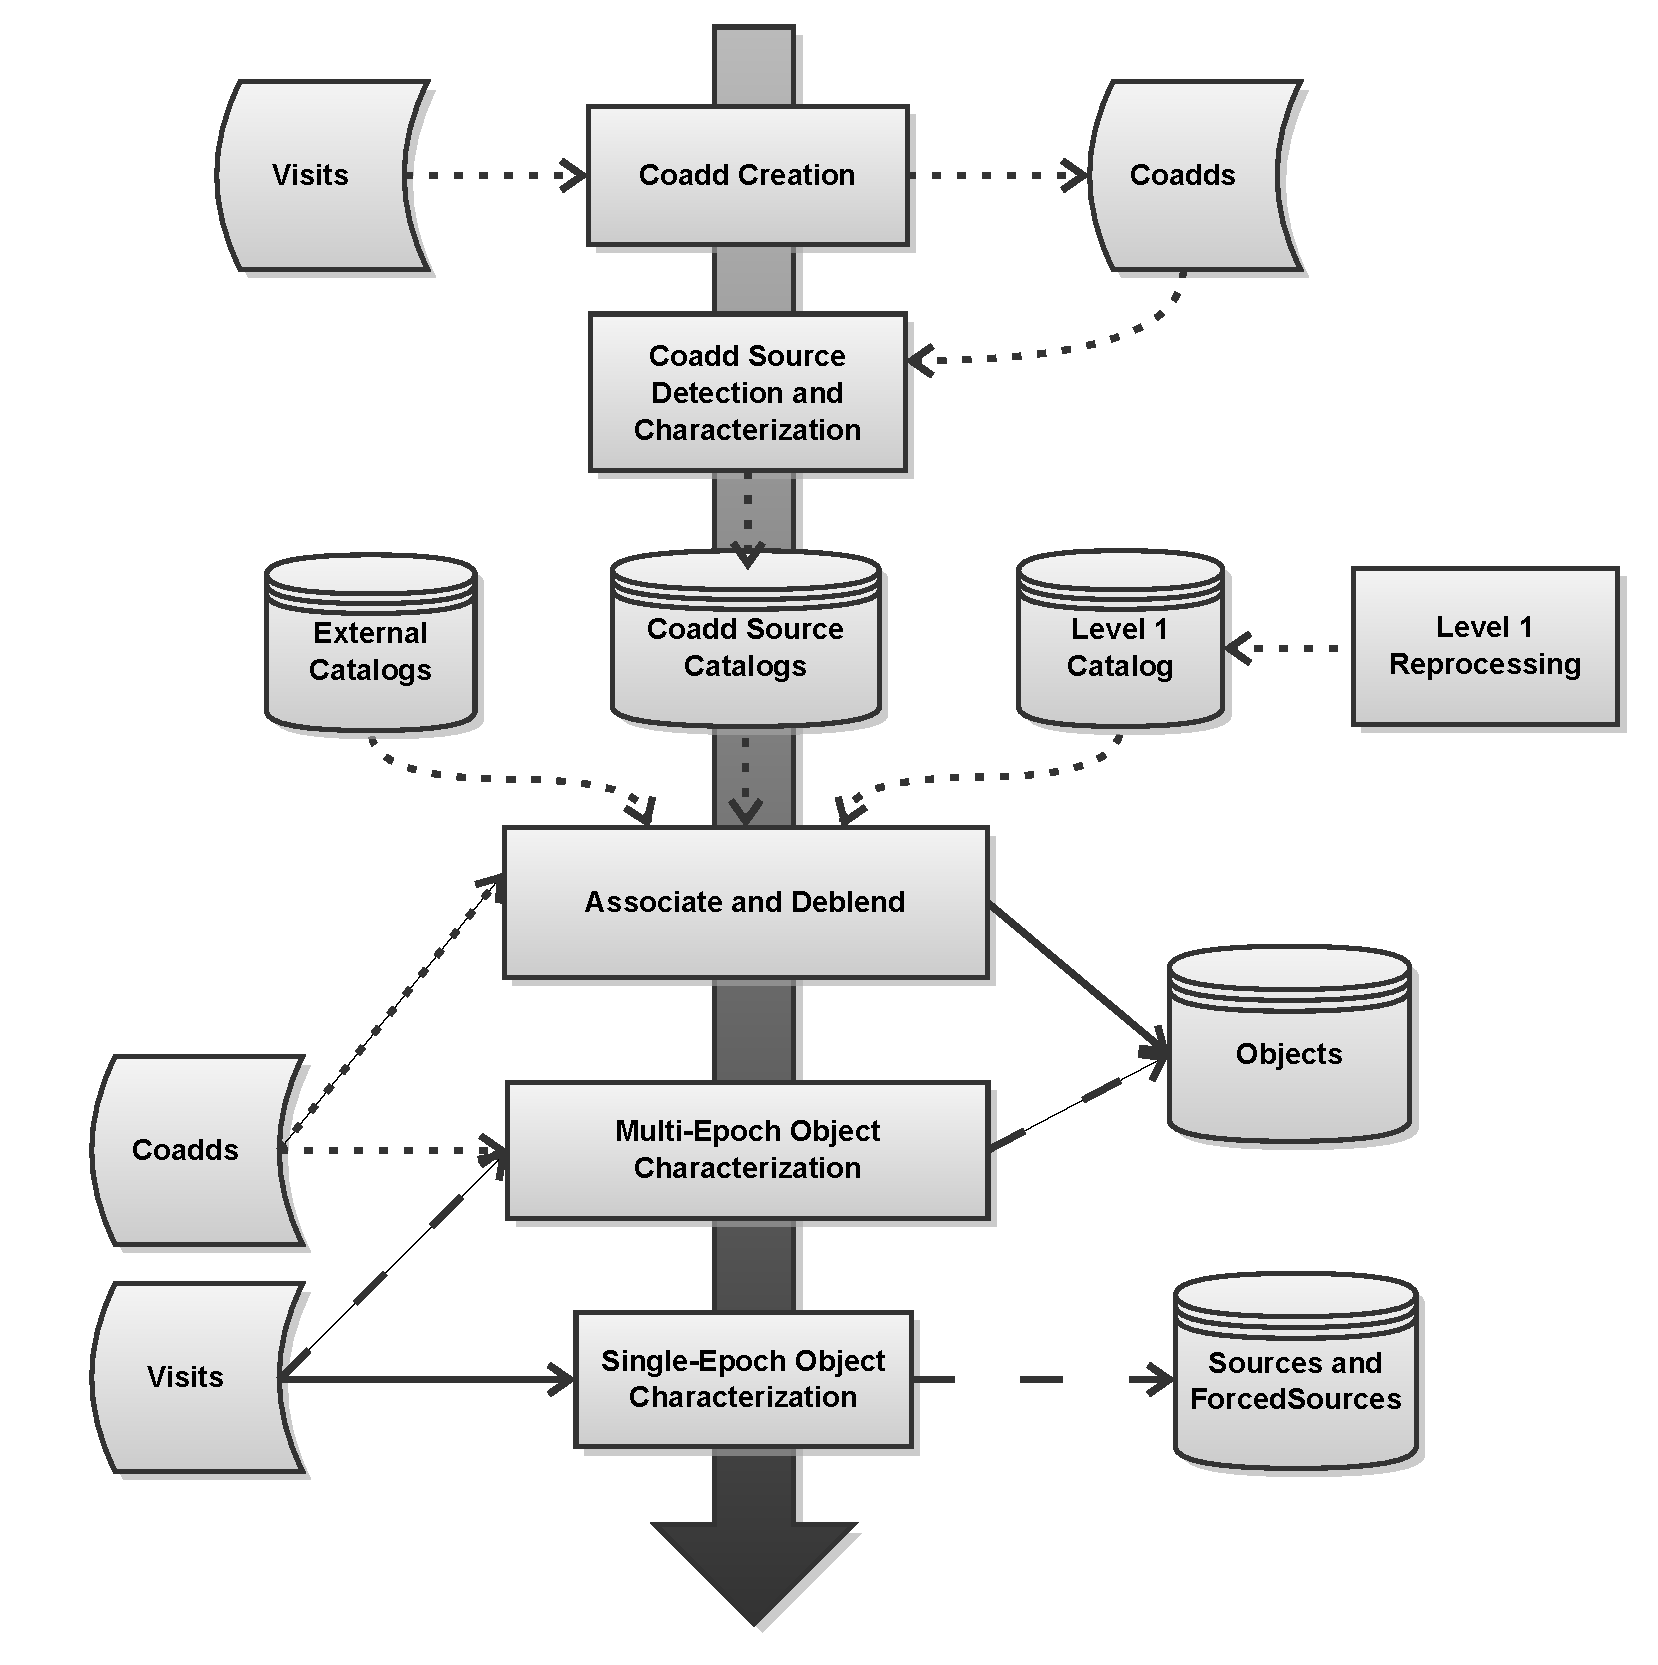
\includegraphics[scale=0.5]{Level_2_Processing_Flowchart}
%    \caption{Level 2 Data Processing Overview\label{fig:level2dp}}
%\end{figure}

Figures~\ref{fig:Pipe1} and \ref{fig:Pipes234}
present a high-level overview of the Level 2 data processing workflow\footnote{Note that some LSST documents refer to \emph{Data Release Processing}, which includes both Level 1 reprocessing (see \S~\ref{sec:l1dbreproc}), and the Level 2 processing described here.}. Logically\footnote{The actual implementation may parallelize these steps as much as possible.}, the processing begins with single-visit image reduction and source measurement, followed by global astrometric and photometric calibration, coadd creation, detection on coadds, association and deblending, object characterization, and forced photometry measurements.

The following is a high-level description of steps which will occur during regular Level 2 data processing
(bullets 1 and 2 below map to pipeline 1, \emph{Single Visit Processing}, in Figure~\ref{fig:Pipe1}, bullet 3 is
pipeline 2, \emph{Image Coaddition}, bullets 4-6 map to pipeline 3, \emph{Coadded Image Analysis}, and
bullet 7 is pipeline 4, \emph{Multi-epoch Object Characterization}):
\begin{enumerate}
    \item \emph{Single Visit Processing}: Raw exposures are reduced to Processed Visit Images, and \Sources are independently detected, deblended, and measured on all visits. Their measurements (instrumental fluxes and shapes) are stored in the \Source table.\dmreq{0267}
    \item \emph{Relative calibration}: The survey is internally calibrated, both photometrically and astrometrically. Relative zero-point and astrometric corrections are computed for every visit.\dmreq{0029} \dmreq{0030} Sufficient data is kept to reconstruct the normalized system response function $\phi_b(\lambda)$ (see Eq.~5, \SRD) at every position in the focal plane at the time of each visit as required by \S~3.3.4 of the \SRD.
    \item \emph{Coadd creation}: Deep, seeing optimized, \dmreq{0279} and short-period per-band coadds\dmreq{0337} are created in $ugrizy$ bands, as well as deeper, multi-color, \dmreq{0281} coadds\footnote{We'll denote the ``band'' of the multi-color coadd as 'M'.}. Transient sources (including Solar System objects, explosive transients, etc), will be rejected from the coadds. See \S~\ref{sec:coadds} for details.
    \item \emph{Coadd source detection}. Sources will be detected on all coadds generated in the previous step.\dmreq{0277} The source detection algorithm will detect regions of connected pixels, known as \emph{footprints}, above the nominal $S/N$ threshold in the \emph{PSF-likelihood image} of the visit. An appropriate algorithm will be run to also detect extended low surface brightness objects
(eg., binned detection algorithm from SDSS).\dmreq{0349}  Each footprint may have one or more \emph{peaks}, and the collection of these peaks (and their membership in the footprints) are the output of this stage.
    \item \emph{Association and deblending}. \dmreq{0275} The next stage in the pipeline, which we will for simplicity just call \emph{the deblender}, will synthesize a list of unique objects. In doing so it will consider the catalogs of \CoaddSources, catalogs of \DIASources, \DIAObjects and \SSObjects detected on difference images, and objects from external
catalogs\footnote{Note that \Sources are not considered when generating the \Object list (given the large
number of visits in each band, the false positives close to the faint end would increase the complexity of
association and deblending algorithms). It is possible for intermittent sources that are detected just above
the faint detection limit of single visits to be undetected in coaddds, and thus to not have a matching \Object.
To enable easy identification of such \Sources, the nearest \Object associated with each \Source, if any, will be recorded.}.\dmreq{0034}

    The deblender will make use of all information available at this stage, including the knowledge of peak positions, bands, time, time variability (from Level 1), Galactic longitude and latitude, etc. The output of this stage is a list of uncharacterized \Objects\footnote{Depending on the exact implementation of the deblender, this stage may also attach significant metadata (eg, deblended footprints and pixel-weight maps) to each deblended \Object record.}.
    \item \emph{Coadd object characterization}.  Object properties such as adaptive moments and aperture fluxes will be measured on the coadds.  These will be stored in additional columns in the \Object table.  Models fit in multi-epoch object characterization will also be fit first to the coadds and stored. \dmreq{0276}
    \item \emph{Multi-epoch object characterization}. A set of predefined model fits and measurements will be performed on each of the \Objects identified in the previous step, \textit{taking all available multi-epoch data into account}. Model fits will be performed using \emph{MultiFit}-type algorithms. Rather than coadding a set of images and measuring object characteristics on the coadd, MultiFit simultaneously fits PSF-convolved models to the objects multiple observations. This reduces systematic errors, improves the overall $S/N$, and allows for fitting of time-dependent quantities degenerate with shape on the coadds (for example, the proper motion). The models we plan to fit will \emph{not} allow for flux variability (see the next item). \dmreq{0275}
    \item \emph{Forced Photometry}. Source fluxes will be measured on every visit, with the position, motion, shape, and the deblending parameters characterized in the previous step kept fixed.
Measurements will be performed on both direct images and difference images.
This process of \emph{forced photometry}, will result in the characterization of the light-curve for each object in the survey. The fluxes will be stored in the \ForcedSource table.\dmreq{0268}
\end{enumerate}

\subsubsection{Object Characterization Measures}
\label{sec:objchar}

Properties of detected objects will be measured as a part of the object characterization step described in the previous section and stored in the \Object table. These measurements are designed to enable LSST ``static sky'' science. This section discusses at a high level which properties will be measured and how those measurements will be performed. For a detailed list of quantities being fit/measured, see the table in \S~\ref{sec:objectTable}.

All measurements discussed in this section deal with properties of \emph{objects}, and will be performed on multi-epoch coadds, or by simultaneously fitting to all epochs. Measurements of sources in individual visits, independent of all others, are described in \S~\ref{sec:sourceMeas}.

To enable science cases depending on observations of non-variable objects in the LSST-observed sky, we plan to measure the following using the MultiFit approach:
%
\begin{itemize}
    \item \emph{Point source model fit}. The observed object is modeled as a point source with finite proper motion and parallax and constant flux (allowed to be different in each band). \dmreq{0276} This model is a good description for non-variable stars and other unresolved sources. Its 11 parameters will be simultaneously constrained using information from all available observations in all bands\footnote{The fitting procedure will account for differential chromatic refraction.}.
    \item \emph{Bulge-disk model fit}. \dmreq{0276} The object is modeled as a sum of a de Vaucouleurs (Sersic $n=4$) and an exponential (Sersic $n=1$) component. This model is intended to be a reasonable description of galaxies\footnote{We may reconsider this choice if a better suited parametrization is discovered while LSST is in Construction.}. The object is assumed not to move\footnote{I.e., have zero proper motion and trigonometric parallax.}. The components share the same ellipticity and center. The model is independently fit to each band. There are a total of 8 free parameters, which will be simultaneously constrained using information from all available epochs for each band. Where there's insufficient data to constrain the likelihood (eg., small, poorly resolved, galaxies, or very few epochs), priors will be adopted to limit the range of its sampling.

We will also explore fitting the galaxy model simultaneously to all bands, with some parameters constrained to be the same or related via a hierarchical model across bands.  As this reduces the number of overall model parameters significantly, we could then consider freeing up other parameters. One likely scenario is that we would allow the bulge and disk ellipticities to differ; another possibility is allowing the Sersic indices of one or both components to vary.  The ultimate determination of which model to use will be driven by empirical tests of the robustness and quality of the fits on both low- and high-redshift galaxies.

\dmreq{0333}
In addition to the maximum likelihood values of fitted parameters and their covariance matrix, a number (currently planned to be $\sim$200, on average\footnote{This choice of the number of independent samples will be verified during Construction.}) of independent samples from the likelihood function will be provided. These will enable use-cases sensitive to departures from the Gaussian approximation, with shear measurement being the primary use case. A permissible descope, in case of insufficient storage, will be not to sample the posterior for $u$ and $y$ bands.

    \item \emph{Standard colors}. \dmreq{0276} Colors of the object in ``standard seeing'' (for example, the third quartile expected survey seeing in the $i$ band, $\sim$0.9\,arcsec) will be measured. These colors are guaranteed to be seeing-insensitive,  suitable for estimation of photometric redshifts\footnote{The problem of optimal determination of photometric redshift is the subject of intense research. The approach we're taking here is conservative, following contemporary practices. As new insights develop, we will revisit the issue.}.

    \item \emph{Centroids}. Centroids will be computed independently for each band using an algorithm similar to that employed by SDSS. Information from all\footnote{Whenever we say \emph{all}, it should be understood that this does not preclude reasonable data quality cuts to exclude data that would otherwise degrade the measurement.} epochs will be used to derive the estimate. These centroids will be used for adaptive moment, Petrosian, Kron, standard color, and aperture measurements. \dmreq{0276}

    \item \emph{Adaptive moments}. Adaptive moments will be computed using information from all epochs, independently for each band. The moments of the PSF realized at the position of the object will be provided as well. \dmreq{0276}

    \item \emph{Petrosian and Kron fluxes}. Petrosian and Kron radii and fluxes will be measured in standard seeing using self-similar elliptical apertures computed from adaptive moments. The apertures will be PSF-corrected and \emph{homogenized}, convolved to a canonical circular PSF\footnote{This is an attempt to derive a definition of elliptical apertures that does not depend on seeing. For example, for a large galaxy, the correction to standard seeing will introduce little change to measured ellipticity. Corrected apertures for small galaxies will tend to be circular (due to smearing by the PSF). In the intermediate regime, this method results in derived apertures that are relatively seeing-independent. Note that this is only the case for \emph{apertures}; the measured flux will still be seeing dependent and it is up to the user to take this into account.}. The radii will be computed independently for each band. Fluxes will be computed in each band, by integrating the light within some multiple of \emph{the radius measured in the canonical band}\footnote{The shape of the aperture in all bands will be set by the profile of the galaxy in the canonical band alone. This procedure ensures that the color measured by comparing the flux in different bands is measured through a consistent aperture. See \url{http://www.sdss.org/dr7/algorithms/photometry.html} for details.} (most likely the $i$ band). Radii enclosing 50\% and 90\% of light will be provided. \dmreq{0276}

    \item \emph{Aperture surface brightness}. Aperture surface brightness will be computed in a variable number\footnote{The number will depend on the size of the source.} of concentric, logarithmically spaced, PSF-homogenized, elliptical apertures, in standard seeing. \dmreq{0276}

    \item \emph{Variability characterization}. Parameters will be provided, designed to characterize periodic and aperiodic variability features \citep{2011ApJ...733...10R}, in each bandpass.
    We caution that the exact features in use when LSST begins operations are likely to be different compared to the baseline described here; this is to be expected given the rapid pace of research in time domain astronomy. However, their \emph{number} is unlikely to grow beyond the present estimate. \dmreq{0276}
\end{itemize}

\subsubsection{Supporting Science Cases Requiring Full Posteriors}

Science cases sensitive to systematics, departures of likelihood from Gaussianity, or requiring user-specified priors, demand knowledge of the shape of the likelihood function beyond a simple Gaussian approximation around the ML value. The estimate of bulge-disk model parameters and the estimate of photometric redshifts are two examples where knowledge of the full posterior is likely to be needed for LSST science cases.\dmreq{0046}\dmreq{0276}

We currently plan to provide this information in two ways: a) by providing independent samples from the likelihood function (in the case of the bulge-disk model), and b) by providing parametric estimates of the likelihood function (for the photometric redshifts). As will be shown in Table~\ref{tbl:objectTable}, the current allocation is $\sim$200 samples (on average) for the bulge-disk model, and $\sim$100 parameters for describing the photo-Z likelihood distributions, per object.

\dmreq{0333}
The methods of storing likelihood functions (or samples thereof) will continue to be developed and optimized throughout Construction and Commissioning. The key limitation, on the amount of data needed to be stored, can be overcome by compression techniques. For example, simply noticing that not more than $\sim$0.5\% accuracy is needed for sample values allows one to increase the number of samples by a factor of $4$. More advanced techniques, such as PCA analysis of the likelihoods across the entire catalog, may allow us to store even more, providing a better estimate of the shape of the likelihood function. In that sense, what is presented in Table~\ref{tbl:objectTable} should be thought of as a \textbf{\emph{conservative estimate}}, which we plan to improve upon as development continues in Construction.

\subsubsection{Source Characterization}
\label{sec:sourceMeas}

Sources will be detected on individual visits as well as the coadds. Sources detected on coadds will primarily serve as inputs to the construction of the master object list as described in \S~\ref{sec:level2dp}, and may support other LSST science cases as seen fit by the users (for example, searches for objects whose shapes vary over time). \dmreq{0277}\dmreq{0267}

The following \Source properties are planned to be measured:
%
\begin{itemize}
    \item \emph{Static point source model fit}. The source is modeled as a static point source. There are a total of 3 free parameters ($\alpha$, $\delta$, flux). This model is a good description of stars and other unresolved sources. \dmreq{0267}

    \item \emph{Centroids}. Centroids are currently planned to be computed using an algorithm similar to that employed by SDSS. These centroids will be used for adaptive moment and aperture magnitude measurements. \dmreq{0267}

    \item \emph{Adaptive moments}. Adaptive moments will be computed. The moments of the PSF realized at the position of the object will be provided as well. \dmreq{0267}

%    \item \emph{Petrosian and Kron fluxes}. Petrosian and Kron radii and fluxes will be measured using elliptical apertures computed from adaptive moments. The apertures will be PSF-corrected and convolved to a canonical circular PSF. Fluxes will be computed in each band, by integrating the light within some multiple of \emph{the radius measured in the same band}\footnote{Note that this is different}. Radii enclosing 50\% and 100\% of light will be provided.

    \item \emph{Aperture surface brightness}. Aperture surface brightness will be computed in a variable number\footnote{The number will depend on the size of the source.} of concentric, logarithmically spaced, PSF-homogenized, elliptical apertures. \dmreq{0267}

%    \item \emph{Bulge-disk model fit}. The object is modeled as a sum of a de Vaucouleurs (Sersic $n=4$) and an exponential (Sersic $n=1$) component. This model is intended to be a reasonable description of galaxies. The object is assumed not to move. The components share the same ellipticity and center. There are a total of 8 free parameters ($\alpha$, $\delta$, $e_1$, $e_2$, $I_{0B}$, $I_{0D}$, $R_{eB}$, $R_{eD}$). Where there's insufficient data to constrain the likelihood (eg., small, poorly resolved, galaxies, or very few epochs), priors will be adopted. Only maximum likelihood values and the covariance matrix will be stored.

\end{itemize}

Note that we do \emph{not} plan to fit extended source Bulge+Disk models to individual \Sources, nor measure per-visit Petrosian or Kron fluxes. These are object properties that are not expected to vary in time\footnote{Objects that \emph{do} change shape with time would, obviously, be of particular interest. Aperture fluxes provided in the \Source table should suffice to detect these. Further per-visit shape characterization can be performed as a Level 3 task.}, and will be better characterized by MultiFit (in the \Object table).
%including the so-called star-galaxy separation (estimation of the probability that a source is resolved, given the PSF).
For example, although a simple extendedness characterization is present in the Source table, star-galaxy separation (an estimate of the probability that a source is resolved, given the PSF) will be better characterized by MultiFit.


\subsubsection{Forced Photometry}
\label{sec:forcedPhotL2}
\dmreq{0268}\dmreq{0287}

\emph{Forced Photometry} is the measurement of flux in individual visits, given a fixed position, shape, and the deblending parameters of an object. It enables the study of time variability of an object's flux, irrespective of whether the flux in any given individual visit is above or below the single-visit detection threshold.

Forced photometry will be performed on all visits, for all \Objects, using both direct images and difference images.
The measured fluxes will be stored in the \ForcedSources table. Due to space constraints, we only plan to measure the PSF flux.

\subsubsection{Crowded Field Photometry}

A fraction of LSST imaging will cover areas of high object (mostly stellar) density. These include the Galactic plane, the Large and Small Magellanic Clouds, and a number of globular clusters (among others).

% LSST does \emph{not} plan to build or deploy algorithms specifically designed for crowded field photometry. \textbf{\emph{Processing these areas using specialist crowded field photometry codes is left to the users as a Level 3 task (see \S~\ref{sec:level3})}}.

LSST image processing and measurement software, although primarily designed to operate in non-crowded regions, is expected to perform well in areas of crowding. The current LSST applications development plan envisions making the deblender aware of Galactic longitude and latitude, and permitting it to use that information as a prior when deciding how to deblend objects. While not guaranteed to reach the accuracy or completeness of purpose-built crowded field photometry codes, we expect this approach will yield acceptable results even in areas of moderately high crowding.

Note that this discussion only pertains to processing of \emph{direct images}. Crowding is not expected to significantly impact the quality of data products derived from \emph{difference images} (i.e., Level 1).

\subsection{The Level 2 Catalogs}

This section presents the contents of key Level 2 catalog tables. As was the case for Level 1 (see \S~\ref{sec:level1db}), here we present the \emph{conceptual schemas} for the most important Level 2 tables (the \Object, \Source, and \ForcedSource tables).
The tables themselves are defined in \citeds{LDM-153}\footnote{The SQL definition itself can be found in the \texttt{cat} package.}.

These convey \emph{what} data will be recorded in each table, rather than the details of \emph{how}. For example, columns whose type is an array (eg., \texttt{radec}) may be expanded to one table column per element of the array (eg., \texttt{ra}, \texttt{decl}) once this schema is translated to SQL. Secondly, the tables to be presented are normalized (i.e., contain no redundant information). For example, since the band of observation can be found by joining a \Source table to the table with exposure metadata, there's no column named \texttt{band} in the \Source table. In the as-built database, the views presented to the users will be appropriately denormalized for ease of use.\dmreq{0332}

\subsubsection{The \Object Table}
\label{sec:objectTable}
\dmreq{0275}

\begin{schema}{\Object Table}{Level 2 Catalog \Object Table}{tbl:objectTable}


objectId & uint64 & ~ & Unique object identifier \\

parentObjectId & uint64 & ~ & ID of the parent \Object this object has been deblended from, if any. \\

radec & double[6][2] & arcsec & Position of the object (centroid), computed independently in each band.
The centroid will be computed using an algorithm similar to that employed by SDSS.\\

radecErr & double[6][2] & arcsec & Uncertainty of \texttt{radec}. \\

psRadecTai & double & time & Point source model: Time at which the object was at position \texttt{psRadec}. \\

psRadec & double[2] & degrees & Point source model: $(\alpha, \delta)$ position of the object at time \texttt{psRadecTai}. \\

psPm & float[2] & mas/yr & Point source model: Proper motion vector.\\

psParallax & float & mas & Point source model: Parallax. \\

psFlux & float[ugrizy] & nmgy & Point source model fluxes\footnote{Point source model assumes that fluxes are constant in each band. If the object is variable, \texttt{psFlux} will effectively be some estimate of the average flux.}.\\

psCov & float[66] & various & Point-source model covariance matrix\footnote{Not all elements of the covariance matrix need to be stored with same precision. While the variances will be stored as 32 bit floats ($\sim$ seven significant digits), the covariances may be stored to $\sim$ three significant digits ($\sim$1\% ).}. \\

psLnL & float & ~ & Natural $log$ likelihood of the observed data given the point source model. \\

psChi2 & float & ~ & $\chi^2$ statistic of the model fit. \\

psNdata & int & ~ & The number of data points (pixels) used to fit the model. \\


bdRadec & double[2][ugrizy] & ~ & B+D model\footnote{Though we refer to this model as ``Bulge plus Disk'', we caution the reader that the decomposition, while physically motivated, should not be taken too literally.}: $(\alpha, \delta)$ position of the object, in each band. \\

bdEllip & float[2][ugrizy] & ~ & B+D model: Ellipticity $(e_1, e_2)$ of the object. \\

bdFluxB & float[ugrizy] & nmgy & B+D model: Integrated flux of the de Vaucouleurs component. \\

bdFluxD & float[ugrizy] & nmgy & B+D model: Integrated flux of the exponential component. \\

bdReB & float[ugrizy] & arcsec & B+D model: Effective radius of the de Vaucouleurs profile component. \\

bdReD & float[ugrizy] & arcsec & B+D model: Effective radius of the exponential profile component. \\

bdCov & float[36][ugrizy] & ~ & B+D model covariance matrix\footnote{See \texttt{psCov} for notes on precision of variances/covariances.}. \\

bdLnL & float[ugrizy] & ~ & Natural $log$ likelihood of the observed data given the bulge+disk model. \\

bdChi2 & float[ugrizy] & ~ & $\chi^2$ statistic of the model fit. \\

bdNdata & int[ugrizy] & ~ & The number of data points (pixels) used to fit the model. \\

bdSamples & float16[9][200][ugrizy] & ~ & Independent samples of bulge+disk likelihood surface. All sampled quantities will be stored with at least $\sim$3 significant digits of precision. The number of samples will vary from object to object, depending on how well the object's likelihood function is approximated by a Gaussian.\\

stdColor & float[5] & mag & Color of the object measured in ``standard seeing''. While the exact algorithm is yet to be determined, this color is guaranteed to be seeing-independent and suitable for photo-Z determinations.\\

stdColorErr & float[5] & mag & Uncertainty of \texttt{stdColor}. \\

Ixx & float & asec$^{2}$ & Adaptive second moment of the source intensity. See \citet{2002AJ....123..583B} for detailed discussion of all adaptive-moment related quantities\footnote{Or \url{http://ls.st/5f4} for a brief summary.}. \\

Iyy & float & asec$^{2}$ & Adaptive second moment of the source intensity. \\

Ixy & float & asec$^{2}$ & Adaptive second moment of the source intensity. \\

Icov & float[6] & asec$^{4}$ & \texttt{Ixx}, \texttt{Iyy}, \texttt{Ixy} covariance matrix. \\

IxxPSF & float & asec$^{2}$ & Adaptive second moment for the PSF. \\

IyyPSF & float & asec$^{2}$ & Adaptive second moment for the PSF. \\

IxyPSF & float & asec$^{2}$ & Adaptive second moment for the PSF. \\

m4 & float[ugrizy] & ~ & Fourth order adaptive moment. \\


petroRad & float[ugrizy] & arcsec & Petrosian radius, computed using elliptical apertures defined by the adaptive moments. \\

petroRadErr & float[ugrizy] & arcsec & Uncertainty of \texttt{petroRad} \\

petroBand & int8 & ~ & The band of the canonical \texttt{petroRad} \\

petroFlux & float[ugrizy] & nmgy & Petrosian flux within a defined multiple of the canonical \texttt{petroRad} \\

petroFluxErr & float[ugrizy] & nmgy & Uncertainty in \texttt{petroFlux} \\

petroRad50 & float[ugrizy] & arcsec & Radius containing 50\% of Petrosian flux. \\

petroRad50Err & float[ugrizy] & arcsec & Uncertainty of \texttt{petroRad50}. \\

petroRad90 & float[ugrizy] & arcsec & Radius containing 90\% of Petrosian flux. \\

petroRad90Err & float[ugrizy] & arcsec & Uncertainty of \texttt{petroRad90}. \\


kronRad & float[ugrizy] & arcsec & Kron radius (computed using elliptical apertures defined by the adaptive moments) \\

kronRadErr & float[ugrizy] & arcsec & Uncertainty of \texttt{kronRad} \\

kronBand & int8 & ~ & The band of the canonical \texttt{kronRad} \\

kronFlux & float[ugrizy] & nmgy & Kron flux within a defined multiple of the canonical \texttt{kronRad} \\

kronFluxErr & float[ugrizy] & nmgy & Uncertainty in \texttt{kronFlux} \\

kronRad50 & float[ugrizy] & arcsec & Radius containing 50\% of Kron flux. \\

kronRad50Err & float[ugrizy] & arcsec & Uncertainty of \texttt{kronRad50}. \\

kronRad90 & float[ugrizy] & arcsec & Radius containing 90\% of Kron flux. \\

kronRad90Err & float[ugrizy] & arcsec & Uncertainty of \texttt{kronRad90}. \\


apNann & int8 & ~ & Number of elliptical annuli (see below). \\

apMeanSb & float[6][\texttt{apNann}] & nmgy/as$^2$ & Mean surface brightness within an annulus\footnote{A database function will be provided to compute the area of each annulus, to enable the computation of aperture flux.}. \\

apMeanSbSigma & float[6][\texttt{apNann}] & nmgy/as$^2$ & Standard deviation of \texttt{apMeanSb}. \\

extendedness & float & ~ & A measure of extendedness, computed using a combination of available moments, or from a likelihood ratio of point/B+D source models (exact algorithm TBD). $extendedness=1$ implies a high degree of confidence that the source is extended. $extendedness=0$ implies a high degree of confidence that the source is point-like. \\

lcPeriodic & float[6~\x~32] & ~ & Periodic features extracted from difference image-based light-curves using generalized Lomb-Scargle periodogram \citep[Table~4,][]{2011ApJ...733...10R}.\\

lcNonPeriodic & float[6~\x~20] & ~ & Non-periodic features extracted from difference image-based light-curves \citep[Table~5,][]{2011ApJ...733...10R}. \\

photoZ & float[2~\x~100] & ~ & Photometric redshift likelihood samples -- pairs of ($z$, $logL$) -- computed using a to-be-determined published and widely accepted algorithm at the time of LSST Commissioning. \\

flags & bit[128] & bit & Various useful flags. \\
\end{schema}


\subsubsection{\Source Table}
\label{sec:sourceTable}

\Source measurements are performed independently on individual visits. They're designed to enable relative astrometric and photometric calibration, variability studies of high signal-to-noise objects, and studies of high SNR objects that vary in position and/or shape (eg., comets).\dmreq{0267}

\begin{schema}{\Source Table}{Level 2 Catalog \Source Table}{tbl:sourceTable}

sourceId & uint64 & ~ & Unique source identifier\footnote{It would be optimal if the source ID is globally unique across all releases. Whether that's realized will depend on technological and space constraints.} \\

ccdVisitId & uint64 & ~ & ID of CCD and visit where this source was measured \\

objectId & uint64 & ~ & ID of the \Object this source was associated with, if any. \\

ssObjectId & uint64 & ~ & ID of the \SSObject this source has been linked to, if any. \\

parentSourceId & uint64 & ~ & ID of the parent \Source this source has been deblended from, if any. \\

xy & float[2] & pixels & Position of the object (centroid), computed using an algorithm similar to that used by SDSS.\\

xyCov & float[3] & ~ & Covariance matrix for \texttt{xy}. \\

radec & double[2] & arcsec & Calibrated ($\alpha$, $\delta$) of the source, transformed from \texttt{xy}.\\

radecCov & float[3] & arcsec & Covariance matrix for \texttt{radec}. \\

apFlux & float & nmgy & Calibrated aperture flux. \\

apFluxErr & float & nmgy &  Estimated uncertainty of \texttt{apFlux}. \\

sky & float & nmgy/asec$^{2}$ & Estimated background (sky) surface brightness at the position (centroid) of the source. \\

skyErr & float & nmgy/asec$^{2}$ & Estimated uncertainty of \texttt{sky}. \\

psRadec & double[2] & degrees & Point source model: $(\alpha, \delta)$ position of the object. \\

psFlux & float & nmgy & Calibrated point source model flux.\\

psCov & float[6] & various & Point-source model covariance matrix\footnote{Not all elements of the covariance matrix will be stored with same precision. While the variances will be stored as 32 bit floats ($\sim$ seven significant digits), the covariances may be stored to $\sim$ three significant digits ($\sim$1\% ).}. \\

psLnL & float & ~ & Natural $log$ likelihood of the observed data given the point source model. \\

psChi2 & float & ~ & $\chi^2$ statistic of the model fit. \\

psNdata & int & ~ & The number of data points (pixels) used to fit the model. \\

Ixx & float & asec$^{2}$ & Adaptive second moment of the source intensity. See \citet{2002AJ....123..583B} for detailed discussion of all adaptive-moment related quantities\footnote{Or \url{http://ls.st/5f4} for a brief summary.}. \\

Iyy & float & asec$^{2}$ & Adaptive second moment of the source intensity. \\

Ixy & float & asec$^{2}$ & Adaptive second moment of the source intensity. \\

Icov & float[6] & asec$^{4}$ & \texttt{Ixx}, \texttt{Iyy}, \texttt{Ixy} covariance matrix. \\

IxxPSF & float & asec$^{2}$ & Adaptive second moment for the PSF. \\

IyyPSF & float & asec$^{2}$ & Adaptive second moment for the PSF. \\

IxyPSF & float & asec$^{2}$ & Adaptive second moment for the PSF. \\

apNann & int8 & ~ & Number of elliptical annuli (see below). \\

apMeanSb & float[\texttt{apNann}] & nmgy & Mean surface brightness within an annulus. \\

apMeanSbSigma & float[\texttt{apNann}] & nmgy & Standard deviation of \texttt{apMeanSb}. \\

extendedness & float & ~ & A measure of extendedness, computed using a combination of available moments
(exact algorithm TBD). $extendedness=1$ implies a high degree of confidence that the source is extended. $extendedness=0$ implies a high degree of confidence that the source is point-like. \\

flags & bit[64] & bit & Various useful flags. \\
\end{schema}


\subsubsection{\ForcedSource Table}
\label{sec:forcedSourceTable}
\dmreq{0268}

\begin{schema}{\ForcedSource Table}{Level 2 Catalog \ForcedSource Table}{tbl:forcedsourceTable}

objectId & uint64 & ~ & Unique object identifier \\

ccdVisitId & uint64 & ~ & ID of CCD and visit where this source was measured \\

% psXY & float[2] & ~ & Location of the measurement, in pixel coordinates\footnote{The precision of the position has to be no greater than 1/100$^\mathrm{th}$ of a pixel. For a 4k$\times$4k CCD, \texttt{psXY} should require no more than 38 bits of storage (or 5 bytes, rounded up)}. \\

psFlux & float & nmgy & Point source model flux on direct image, if performed.\\

psFluxErr & float & nmgy & Point source model flux error,  stored to 1\% precision.\\

psDiffFlux & float & nmgy & Point source model flux on difference image, if performed.\\

psDiffFluxErr & float & nmgy & Point source model flux error,  stored to 1\% precision.\\

% bdFlux & float & nmgy & Bulge+disk model flux.\\

% bdFluxErr & float & nmgy & Bulge+disk model flux error, stored to 1\% precision.\\

flags & bit[8] & bit & Various useful flags. \\
\end{schema}


\subsection{Level 2 Image Products}

\subsubsection{Visit Images}

\dmreq{0065}

Raw exposures, including individual snaps, and Processed Visit Images will be made available for download as FITS files. They will be downloadable both through a human-friendly Science User Interface, as well as using machine-friendly APIs.

Required calibration data,\dmreq{0130} processing metadata,\dmreq{0298} and all necessary image processing software will be provided to enable the user to generate bitwise identical processed images from raw images\footnote{Assuming identically performing software and hardware configuration.}.\dmreq{0308}

\subsubsection{Calibration Data}

All calibration frames (darks, flats, biases, fringe, etc.)\dmreq{0130} will be preserved and made available for download as FITS files.\dmreq{0065}\dmreq{0298}

All auxiliary telescope data, both raw (images with spectra) and processed (calibrated spectra, derived atmosphere models), will be preserved and made available for download.

\subsubsection{Coadded Images}
\label{sec:coadds}

In course of Level 2 processing, multiple classes and numerous of coadds will be created\footnote{See \citeds{LDM-151} for more details.}:

\begin{itemize}
    \item A set of \emph{deep coadds}.\dmreq{0279} One deep coadd will be created for each of the $ugrizy$ bands, plus a seventh, deeper, multi-color coadd.\dmreq{0281} These coadds will be optimized for a reasonable combination of depth (i.e., employ no PSF matching) and resolution (i.e., visits with significantly degraded seeing may be omitted). Transient sources (including Solar System objects, explosive transients, etc), will be removed. Care will be taken to preserve the astrophysical backgrounds\footnote{For example, using ``background matching'' techniques \citep{DMTN-035}}.

    The six per-band coadds will be kept indefinitely and made available to the users.\dmreq{0334} \emph{Their primary purpose is to enable the end-users to apply alternative object characterization algorithms, perform studies of diffuse structures, and for visualization}.

    \item A set of \emph{best seeing} coadds. One deep coadd will be created for each of the $ugrizy$ bands, using only the best seeing data (for example, using only the first quartile of the realized seeing distribution). These will be built to assist the deblending process. These coadds will be kept indefinitely and made available to the users. \dmreq{0330}\dmreq{0334}

    \item A set of \emph{short-period} coadds.\dmreq{0337} These will comprise of multiple (ugrizyM) sets of yearly and multi-year coadds. Each of these sets will be created using only a subset of the data, and otherwise share the characteristics of the deep coadds described above. These are designed to enable detection of long-term variable or moving\footnote{For example, nearby high proper motion stars.} objects that would be ``washed out'' (or rejected) in full-depth coadds. \textbf{We \em do not plan to keep and make these coadds available}. We will retain and provide sufficient metadata for users to re-create them using Level 3 or other resources.\dmreq{0298}\dmreq{0311}

    \item One (ugrizyM) set of PSF-matched coadds.\dmreq{0335} These will be used to measure colors and shapes of objects at ``standard'' seeing. \textbf{\emph{We do not plan to keep and make these coadds available}}. We will retain and provide sufficient metadata for users to re-create them using Level 3 or other resources.
\end{itemize}

The exact details of which coadds to build, and which ones to keep, can change during Construction without affecting the processing system design as the most expensive operations (raw image input and warping) are constant in the number of coadds produced. The data management system design \emph{is} sensitive to the total \emph{number and size} of coadds to be \emph{kept} -- these are the relevant constraining variables.

We reiterate that \textbf{not all coadds will be kept and served to the public}\footnote{The coadds are a major cost driver for storage. LSST Data Management system is currently sized to keep and serve seven coadds, \emph{ugrizyM}, over the full footprint of the survey.}, though sufficient metadata will be provided to users to recreate them on their own. Some coadds may be entirely ``virtual'': for example, the PSF-matched coadds could be implemented as ad-hoc convolutions of postage stamps when the colors are measured.\dmreq{0311}

We \emph\textbf{will} retain smaller sections of all generated coadds, to support quality assessment and targeted science.\dmreq{0338} Retained sections may be positioned to cover areas of the sky of special interest such as overlaps with other surveys, nearby galaxies, large clusters, etc.

\subsection{Data Release Availability and Retention Policies}
\label{sec:retention}

Over 10 years of operations, LSST will produce eleven data releases: two for the first year of survey operations, and one every subsequent year. Each data release will include reprocessing of all data from the start of the survey, up to the cutoff date for that release.

The contents of data releases are expected to range from a few PB (DR1) to $\sim$70\,PB for DR11 (this includes the raw images, retained coadds, and catalogs). Given that scale, it is not feasible to keep all data releases loaded and accessible at all times.

Instead, \textbf{\emph{only the contents of the most recent data release, and the penultimate data release will be kept on fast storage and with catalogs loaded into the database}}. \dmreq{0313} Statistics collected by prior surveys (eg., SDSS) show that users nearly always prefer accessing the most recent data release, but sometimes may use the penultimate one (this is especially true just after the publication of a new data release). Older releases are used rarely.

To assist with data quality monitoring and assessment \textbf{\emph{small, overlapping, samples of data from older releases will be kept loaded in the database}}.\dmreq{0339} The sample size is expected to be on order of $\sim$1-5\% of the data release data, with larger samples kept early on in the survey. The goal is to allow one to test how the reported characterization of the same data varies from release to release.

Older releases will be archived to mass storage (tape). The users \textbf{\emph{will not be able to perform database queries against archived releases}}. They will be made available as bulk downloads in some common format (for example, FITS binary tables). Database software and data loading scripts will be provided for users who wish to set up a running copy of an older (or current) data release database on their systems.
\dmreq{0077}\dmreq{0300}

All raw data used to generate any public data product (raw exposures, calibration frames, telemetry, configuration metadata, etc.) will be kept and made available for download. \dmreq{0309}\dmreq{0346}

\begin{openissues}
\subsection{Open Issues}

What follows is a (non-exhaustive) list of issues, technical and scientific, that are still being discussed and where changes are possible. The estimate of the time by which a decision should be made is noted in parentheses.

\begin{itemize}
    \item \emph{Is our approach to crowded field photometry satisfactory?} Is there another, given the budget and schedule constraints? (FDR)

    \item \emph{What is the definition of a crowded field?} This is related to the question of when is LSST photometry allowed to deviate from \SRD specs due to crowding. (FDR)

    \item \emph{Are we going to provide additional characterization for large galaxies (isophote twists, bars, etc)?} How far should (and can) we go with ``large'' galaxy characterization. Measures like isophote twists, Gini coefficients, etc. This is now considered to be Level 3, but it's likely at least a portion of it belongs to Level 2 -- assuming we're given a set of well-defined morphology measures. Input from the galaxies (and strong lensing?) Collaborations would be useful. (CONSTRUCTION)

    \item \emph{Which coadds to we keep and serve to the public?} Probably non-PSF matched coadds with CoaddPsf (aka. StackFit PSF). PSF-matched coadds are another option and may be easier for the users to work with. (CONSTRUCTION)

    \item \emph{What is the primary use-case for retained coadds?} These are the set of coadds (one per band) that we'll serve to the users. For example, should the primary purpose of deep coadds be the study of diffuse structures (in which case we may prefer to optimize depth at the cost of degrading the seeing), or is it to enable alternative studies of object shapes, where the resolution (and minimization of systematics) is paramount? This is very much related to the question above. (CONSTRUCTION)

    \item \emph{Do we need both Kron and Petrosian fluxes?} These are intimately related to aperture fluxes, and given aperture fluxes in multiple apertures may be even derived from these. (OPERATIONS)

    \item \emph{Do we need multiple estimates of object centroids?} The document currently assumes that the model-independent centroiding algorithm, the point source model fit, and the extended source model fit, don't necessarily need to agree on the location of the center of an object. This is true in general. However, it has been pointed out that when they do not agree, the associated flux measurement is meaningless anyway. (OPERATIONS)

\end{itemize}
\end{openissues}

\clearpage

\section{Level 3 Data Products and Capabilities}
\label{sec:level3}

\emph{Level 3 capabilities} are envisioned to enable science cases that would greatly benefit from co-location of user processing and/or data within the LSST Archive Center. The high-level requirement for Level 3 is established in \S~3.5 of the LSST \SRD.
\ossreq{0140}

Level 3 capabilities include three separate deliverables:
%
\begin{enumerate}
    \item Level 3 Data Products and associated storage resources
    \item Level 3 processing resources, and
    \item Level 3 programming environment and framework
\end{enumerate}
%
Many scientists' work may involve using two or all three of them in concert, but they can each be used independently. We describe each one of them in the subsections to follow.

\subsection{Level 3 Data Products and Associated Storage Resources}

\dmreq{0290}
These are data products that are generated by users \emph{on any computing resources anywhere} that are then brought to an LSST Data Access Center (DAC) and stored there. The hardware for these capabilities includes the physical storage and database server resources at the DAC to support them.

For catalog data products, there is an expectation that they can be ``federated'' with the Level 1 (L1) and Level 2 (L2) catalogs to enable analyses combining them.  Essentially this means that either the user-supplied tables include keys from the L1/L2 catalogs that can be used for key-equality-based joins with them (example: a table of custom photometric redshifts for galaxies, with a column of object IDs that can be joined to the L2 Object catalog), or that there are columns that can be used for spatial (or temporal, or analogous) joins against L1/L2 tables. The latter implies that such L3 table's columns must be in the same coordinate system and units as the corresponding L1/L2 columns.
\dmreq{0123}
\dmreq{0124}

There is no requirement that Level 3 data products (L3DPs) are derived from L1 or L2 other than that they be joinable with them.  For instance, a user might have a catalog of radio sources that they might want to bring into federation with the LSST catalogs. That can be thought of as a Level 3 Data Product as long as they have ``LSST-ized'' it by ensuring compatibility of coordinate, time, measurement systems, etc.  Nevertheless, we do expect the majority of L3DPs to be derived from processed LSST data.

There could also be L3 image data products; for example, user-generated coadds with special selection criteria or stacking algorithms (eg. the so-called shift \& stack algorithm for detecting moving objects).
\dmreq{0127}

Any L3DP may have access controls associated with it, restricting read access to just the owner, to a list of people, to a named group of people, or allowing open access.\dmreq{0340}

The storage resources for L3DPs come out of the \SRD requirement for 10\% of LSST data management capabilities to be devoted to user processing. In general, they are likely to be controlled by some form of a ``space allocation committee''.  Users will probably have some small baseline automatic allocation, beyond which a SAC proposal is needed. The SAC may take into account scientific merit, length of time for which the storage is requested, and openness of the data to others, in setting its priorities.
\dmreq{0119}

It is to be decided whether users will be required to provide the code and/or documentation behind their L3DPs, or whether the SAC may include the availability of this supporting information in its prioritization.  Obviously if a user intends to make a L3DP public or publish it to a group it will be more important that supporting information be available.

Level 3 data products that are found to be generally useful can be migrated to Level 2.
This is a fairly complex process that ultimately involves the project taking responsibility for supporting and running LSST-style code that implements the algorithm necessary to produce the data product (it's not just relabeling an existing L3DP as L2).  The project will provide necessary support for such migrations.

\subsection{Level 3 Processing Resources}
\dmreq{0119}

These are project-owned computing resources located at the DACs.  They are available for allocation to all users with LSST data rights.  They may be used for any computation that involves the LSST data and advances LSST-related science. The distinctive feature of these computing resources is that they are located with excellent I/O connections to the image and catalog datasets at Level 1 and Level 2. There may be other co-located but \emph{not} project-owned, resources available at the LSST DACs\footnote{For example, the U.S. DAC will be located at the National Petascale Facility building at NCSA, adjacent to the Blue Waters supercomputer.}; their use is beyond the scope of this document, except to note that reasonable provisions will be made to ensure it \emph{is} possible to use them to process large quantities of LSST data.

Level 3 processing resources will, at least, include systems that can carry out traditional batch-style processing, probably similarly configured to those LSST will be using for the bulk of data release production processing.  It is to be determined whether any other flavors of hardware would be provided, such as large-memory machines; this is likely to be driven by the project need (or lack thereof) for such resources.

There will be a time allocation committee (TAC) for these resources.  Every LSST-data-rights user may get a small default allocation (enough to run test jobs).  Substantial allocations will require a scientific justification.  Priorities will be based on the science case and, perhaps, also on whether the results of the processing will be released to a larger audience.  Requests must specify what special flavors of computing will be needed (e.g., GPUs, large memory, etc.).

A fairly standard job control environment (like Condor), will be available, and users will be permitted to work with it at a low, generic level. They will not be required to use the higher levels of the LSST process control middleware (but they may; see \S~\ref{sec:l3framework}).

These processing resources can be available for use in any clearly LSST-related scientific work.  It is not strictly required that they be used to process LSST data, in this context.  For instance, it could be acceptable to run special types of cosmological simulations that are in direct support of an LSST analysis, \emph{if the closeness to the data makes the LSST facility uniquely suitable for such work}. The TAC will take into account in its decisions whether proposed work makes good use of the enhanced I/O bandwidth available to LSST data on these systems.

\subsection{Level 3 Programming Environment and Framework}
\label{sec:l3framework}
\dmreq{0125}
\dmreq{0128}

As a part of the Level 3 Programming Environment and Framework, the LSST will make available the LSST software stack to users, to aid in the analyses of LSST data. This includes all code implementing the core processing algorithms (image characterization and manipulation, building of coadds, image differencing, object detection, object characterization, moving object detection, etc.), the middleware necessary to run those codes at large scale, as well as the LSST database management system.
\dmreq{0033}
\dmreq{0032}
\dmreq{0308}

These analyses could be done on LSST-owned systems (i.e., on the Level 3 processing resources) but also on a variety of supported external systems.  We will aim to support common personal Unix flavors (for example, common distributions of Linux and Mac OS X) as well as commonly used cluster and HPC environments.  The vision is to enable relatively straightforward use of major national systems such as XSEDE or Open Science Grid, as well as some common commercial cloud environments.  The decision of which environments to support will be under configuration control and we will seek advice from the user community.  We cannot commit to too many flavors.  In-kind contributions of customizations for other environments will be welcome and may provide a role for national labs.

The Level 3 environment is intended, when put to fullest use, to allow users to run their own productions-like runs on bulk image and/or catalog data, with mechanisms for creating and tracking large groups of jobs in a batch system.

The Level 3 environment, in asymptopia, has a great deal in common with the environment that the Project will use to build the Level 2 data releases. It is distinct, however, as supporting it as a tool meant for the end-users imposes additional requirements:
%
\begin{itemize}
    \item In order to be successful as a \emph{user} computing environment, it needs to be easy to use. Experience with prior projects\footnote{For example, BaBar.} has shown that if the production computing environment is not envisioned from the start as being shared with users, it will likely evolve into an experts-only tool that is too complicated, or too work-hardened, to serve users well.
    \item While it is desirable for the production computing to be portable to Grid, cloud, etc. resources, this option might not be exercised in practice and could atrophy.  For the user community, it's a far more central capability. Early community engagement is therefore key to developing and maintaining these capabilities.
    \item Not all the capabilities of the LSST production environment need necessarily be exported to the users. LSST-specific capabilities associated with system administration, for instance, are not of interest to end-users.
\end{itemize}

%While the three "Level 3"s are often used together, all eight combinations make sense, so they are truly independent:
%
%                    !L3DP                                  L3DP
%
%!L3proc, !L3env     Analyze LSST data on your own          ... and generate data products
%                    computer, grid, cloud, starting        to be federated with the L1 & L2DPs at a DAC, returned
%                    from public export formats             to the DAC in a supported export/import format like
%                    (FITS, VOTable, csv)                   VOTable, FITS binary table
%
%!L3proc, L3env      Analyze LSST data on your own          ... and read existing L3DPs, or
%                    computer, grid, cloud, starting        generate data products to be federated
%                    from the results of LSST query APIs    with the L1 & L2DPs at a DAC, returned to the
%                    or from public export formats, and     DAC using an LSST API or through supported
%                    using the LSST stack to support the    export/import formats
%                    analyses (e.g., using afw to deal
%                    with image data) and organize the
%                    division of the work into jobs
%
%L3proc, L3env       Analyze LSST data on LSST hardware     ... and read existing L3DPs, or
%                    at a DAC in the LSST framework, in a   generate data products to be federated
%                    way very much like what DRP does,      with the L1 & L2DPs at that DAC, very likely
%                    except with user code doing the        using essentially the same APIs used by DRP to
%                    science.                               store its outputs.
%
%L3proc, !L3env      Analyze LSST data on LSST hardware     ... and read existing L3DPs, or
%                    with essentially non-LSST-flavored     generate data products to be federated
%                    code.  LSST hardware just used as a    with the L1 & L2DPs at that DAC, through a
%                    generic computing resource, but the    supported export/import data format.
%                    proximity to the data may still be
%                    crucial to the work.
%
%Obviously there is a continuum from the extreme "!L3env" case of using no LSST code at all in the analysis, to the maximum "L3env" case of using virtually the entire stack, from afw through the process control middleware.

\subsection{Migration of Level 3 data products to Level 2}

\begin{itemize}
    \item For the migration to be considered, the creator of the L3DP will need to agree to make their data product public to the entire LSST data-rights community, along with supporting documentation and code. The code at first need not be in the LSST framework or even in an LSST-supported language.
    \item If the original proponent wrote her/his code in the C++/Python LSST stack environment (the ``Level 3 environment''), it will be easier to migrate it to Level 2 (though, obviously, using the same languages/frameworks does not guarantee that the code is of production quality).
    \item If the original code was written in another language or another data processing framework, the project may consider rewriting it to required LSST standards.
    \item Taking on a new Level 2 DP means that the project is committing to code maintenance, data quality review, space allocation, and continuing production of the new L2DP through DR11.
\end{itemize}

\clearpage

\section{Data Products for Special Programs}
\label{sec:specialProgs}

\lsrreq{0075}
LSST Survey Specifications (LSST \SRD, \S~3.4) specify that 90\% of LSST observing time will be spend executing the so-called ``universal cadence''. These observations will result in Level 1 and 2 data products described earlier in this document.

The remaining 10\% of observing time will be devoted to special programs, obtaining improved coverage of interesting regions of observational parameter space. Examples include very deep ($r\sim26$, per exposure) observations, observations with very short revisit times ($\sim$1 minute), and observations of ``special'' regions such as the Ecliptic, Galactic plane, and the Large and Small Magellanic Clouds. A third type of survey, micro-surveys, that would use about 1\% of the time, may also be considered.

The details of these special programs or micro surveys are not yet defined\footnote{The initial complement is expected to be defined and selected no later than Science Verification.}. Consequently, the specifics of their data products are left undefined at this time. Instead, we just specify the \emph{constraints} on these data products, given the adopted Level 1/2/3 architecture. It is understood that no special program will be selected that does not fit these constraints\footnote{Or will come with additional, external, funding, capabilities, and/or expertise.}. This allows us to size and construct the data management system, without knowing the exact definition of these programs this far in advance.

Processing for special programs will make use of the same software stack and computing capabilities as the processing for universal cadence.\dmreq{0320} The programs are expected to use no more than $\sim$10\% of computational and storage capacity of the LSST data processing cluster. When special products include time domain event alerts, their processing shall generally be subject to the same latency requirements as Level 1 data products.\dmreq{0321}\dmreq{0344}\reqparam{OTT1}

For simplicity of use and consistency, the data products for special programs will be stored in databases separate from the ``main'' (Level 1 and 2) databases. The system will, however, allow for simple federation with Level 1/2/3 data products (i.e., cross-queries and joins).\dmreq{0322}

As a concrete example, a data product complement for a ``deep drilling'' field designed for supernova discovery and characterization may consist of: i) alerts to events discovered by differencing the science images against a special deep drilling template, ii) a Level 1-like database iii) one or more ``nightly co-adds'' (co-adds built using the data from the entire night), produced and made available within $\sim$24 hours\reqparam{L1PublicT}, and iv) special deep templates, built using the best recently acquired seeing data, produced on a fortnightly cadence.

Note that the data rights and access rules apply just as they would for for Level 1/2/3. For example, while generated event alerts (if any) will be accessible world-wide, the image and catalog products will be restricted to users with LSST data rights.

\bibliography{dpdd,lsst,refs_ads}


\clearpage
\appendix
\section{Appendix: Conceptual Pipeline Design \label{sec:scipi}}

A high-level conceptual overview of the LSST image processing science pipelines is illustrated
in Figure~\ref{fig:Detail1}. The pipeline definitions presented here are driven by their inputs,
outputs and processing steps; they do \textit{not} describe exact boundaries in the actual implemention
code, execution, or development responsibilities within the Project.
Processing from pipelines marked with 1, 2, and 5-8 is executed every day when new data are taken
to produce Level 1 Data Products. Annual Data Release processing includes pipelines 1-6 and 8
(everything except Alert production). These main conceptual steps in LSST image processing
include the following pipelines (enumeration in this list corresponds to enumeration in Figure~\ref{fig:Detail1}
but note that these steps can be interleaved in the actual processing flow):
\begin{enumerate}
\item \textit{Single Visit Processing} pipeline (Figure~\ref{fig:Pipe1}) produces calibrated and
characterized single-visit images from raw snaps. The main processing steps include instrumental
signature removal, background estimation, source detection, deblending and measurements,
point spread function estimation, and astrometric and photometric calibration.
\item \textit{Image Coaddition} pipeline (Figure~\ref{fig:Pipes234}) produces coadded images
of different flavors (optimized for depth, seeing, etc.) from an ensemble of single-visit images.
\item \textit{Coadded Image Analysis} pipeline (Figure~\ref{fig:Pipes234}) defines the \Object list
and performs initial measurements on coadded images.
\item \textit{Multi-epoch Object Characterization} pipeline (Figure~\ref{fig:Pipes234}) fits a library
of image models to a set of Footprints of an \Object family, measures additional quantities (e.g.,
the profile surface brightness in a series of annuli) not captured by those models, and performs
Forced Photometry. All these measurements are performed on single-visit images (direct and
difference images) and for all \Objects.
\item \textit{Image Differencing} pipeline (Figure~\ref{fig:Pipes567}) produces difference images
from a single-visit and coadded (template) images.
\item \textit{Difference Image Analysis} pipeline (Figure~\ref{fig:Pipes567}) updates
\DIAObject and \SSObject lists with new \DIASources detected on processed difference image,
fits a library of image models to Footprints of these \DIASources, and for all \DIAObjects
overlapping the difference image it performs Forced Photometry and recomputes summary quantities.
During nightly Level 1 processing, this pipeline also performs Forced Photometry
for all new \DIAObjects on difference images from the last 30 days\reqparam{precoveryWindow}.
\item \textit{Alert Generation and Distribution} pipeline (Figure~\ref{fig:Pipes567}) uses updated
\DIAObjects and \DIASources to generate and distribute \Alerts (which also include postage stamp
images of the \DIASource in difference image and coadded template image).
\item \textit{Moving Object Processing} pipeline (MOPS, Figure~\ref{fig:Pipe8})) combines all
un-associated \DIASources into plausible \SSObjects and estimates their orbital parameters.
The three main pipeline stages include associating new \DIASources with known \SSObjects,
discovering new \SSObjects, and orbit refinement and management.
\end{enumerate}

Further details about the pipeline design and implementation are available from the LSST
document \citeds{LDM-151}.

\begin{figure}[!t]
    \centering
    \vskip -0.1in
    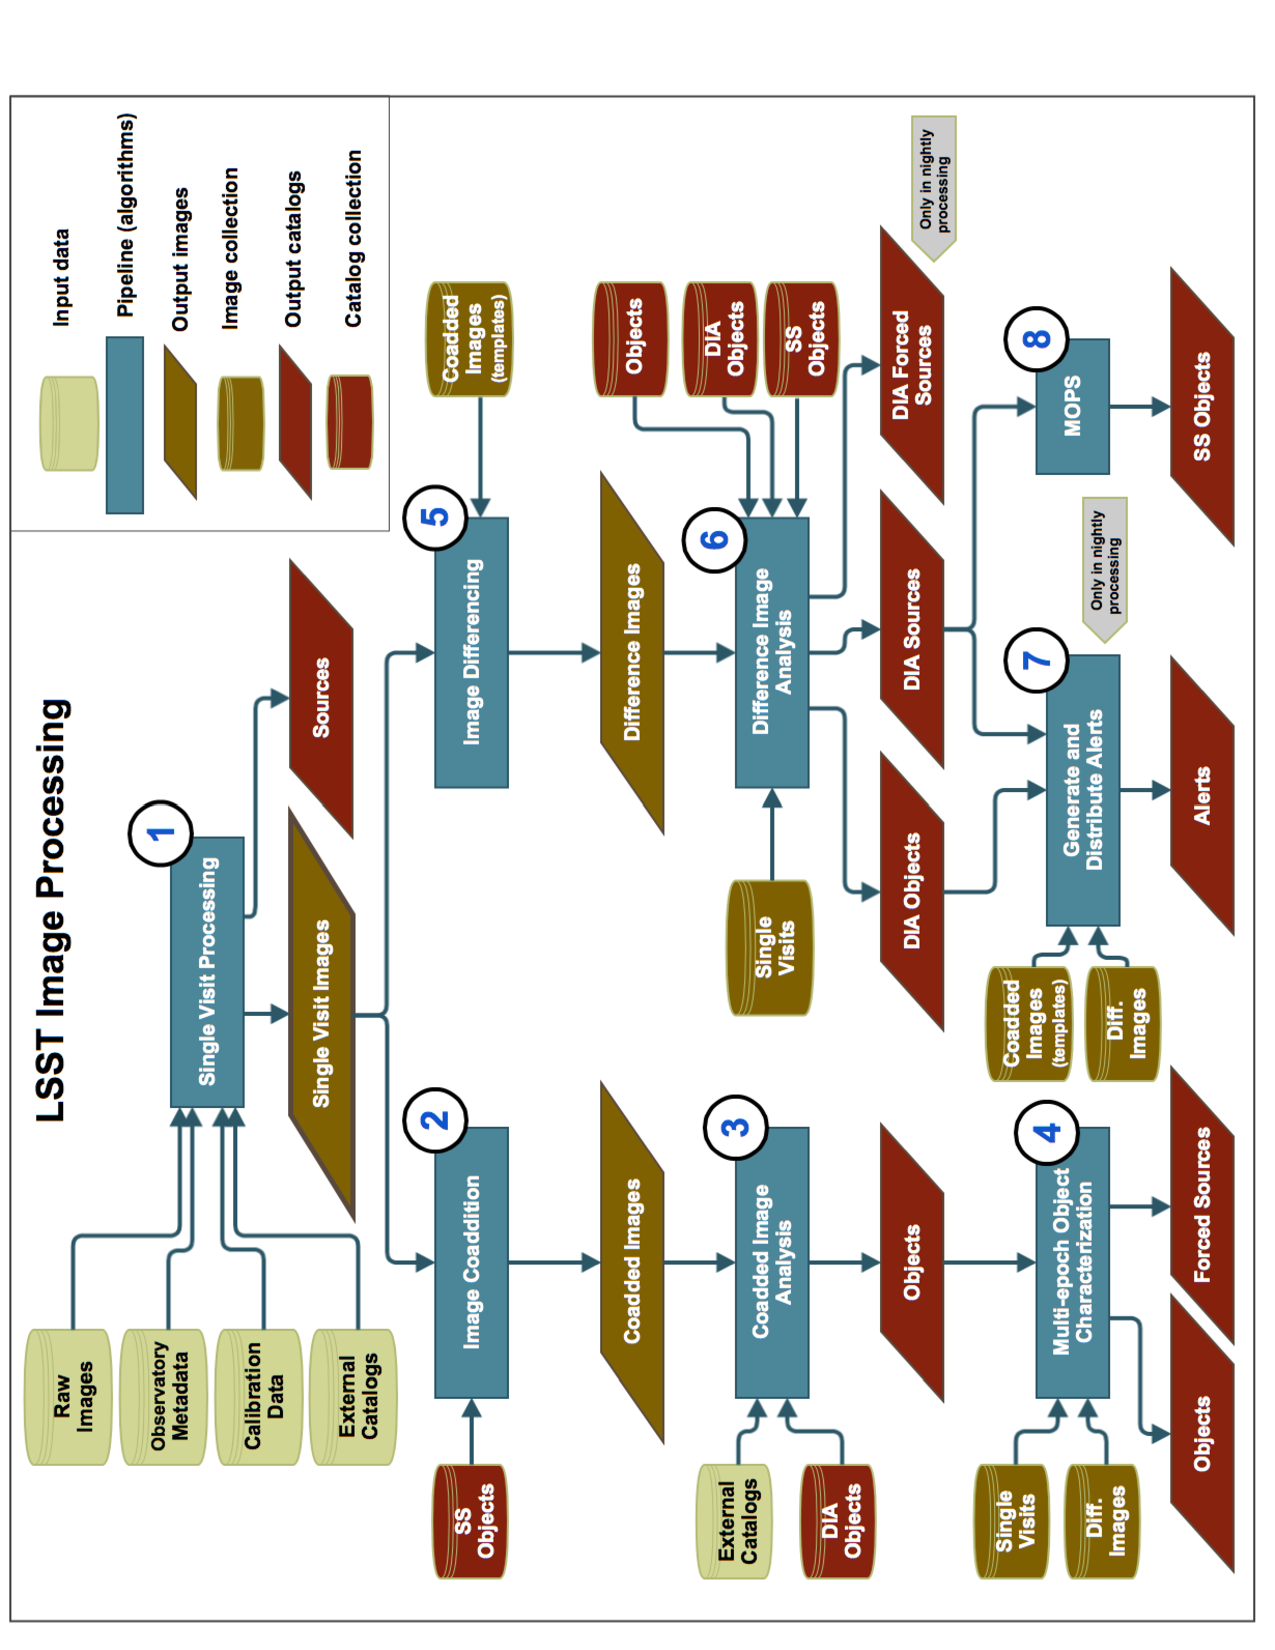
\includegraphics[scale=0.515, angle=270]{gliffy/LSSTimageProcessingDetail1}
    \vskip -0.1in
    \caption{Illustration of the conceptual design of LSST science pipelines for imaging processing.\label{fig:Detail1}}
\end{figure}


\begin{figure}[!t]
    \centering
    \vskip -1.1in
    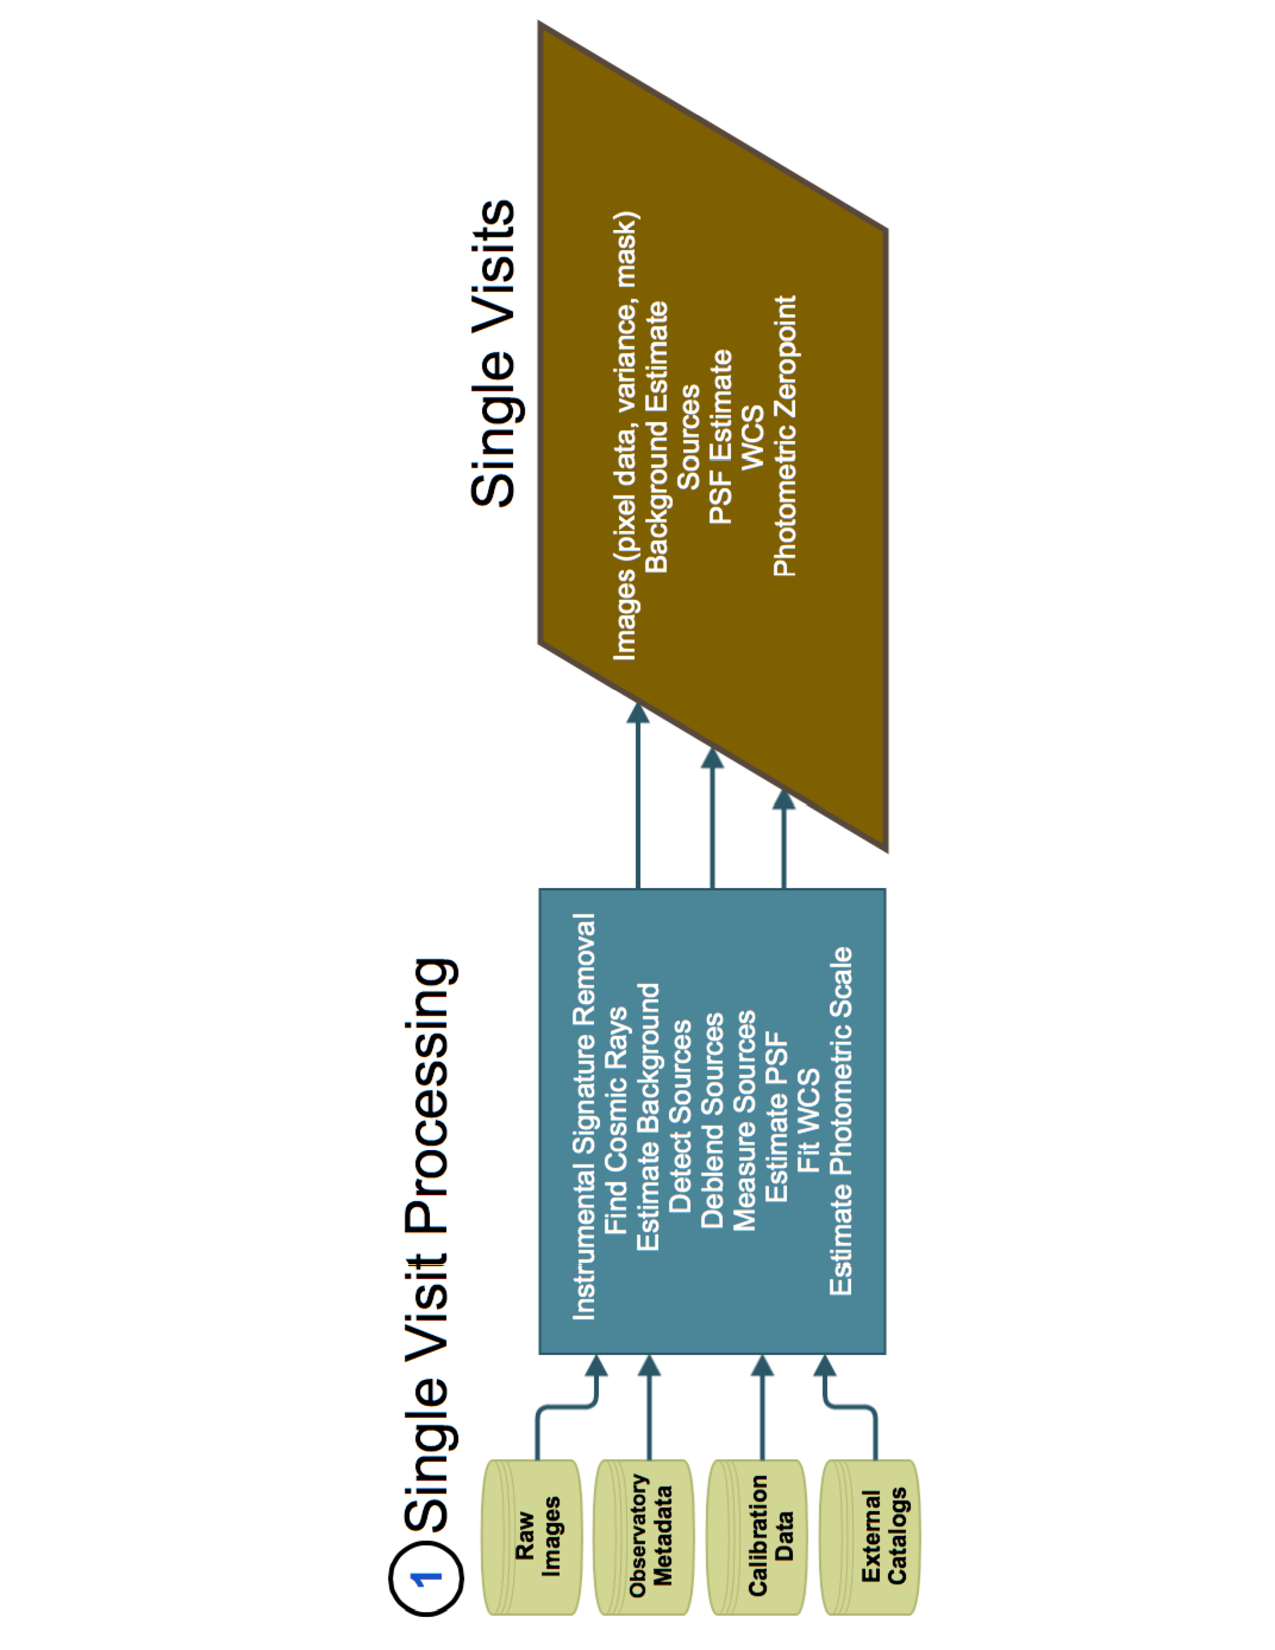
\includegraphics[scale=0.505, angle=270]{gliffy/SingleVisitProcessing}
    \vskip -1.1in
    \caption{Illustration of the conceptual algorithm design for Single Visit Processing pipeline.\label{fig:Pipe1}}
\end{figure}

\begin{figure}[!th]
    \centering
    \vskip -0.2in
    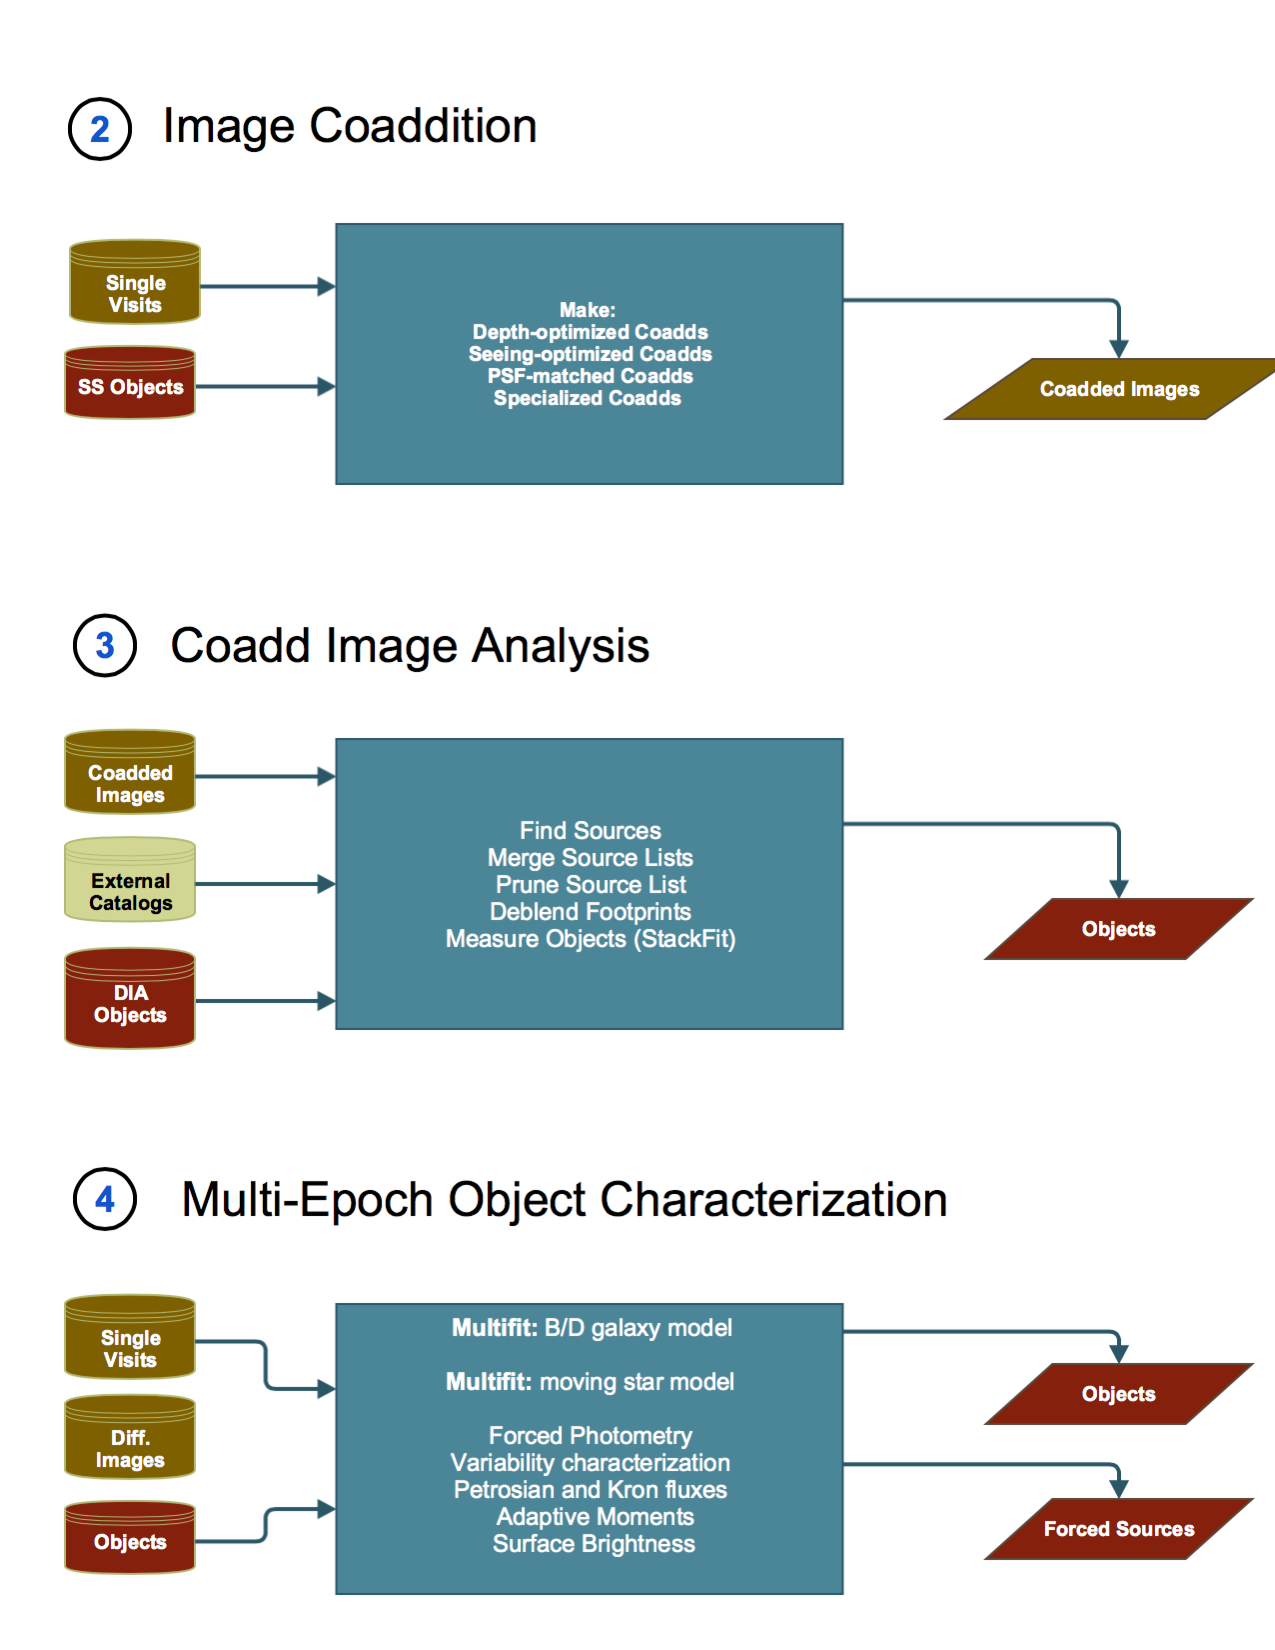
\includegraphics[scale=0.535]{gliffy/CoaddedImageProcessing}
    \vskip -0.2in
    \caption{Illustration of the conceptual algorithm design for Image Coaddition, Coadded Image Analysis,
     and Multi-epoch Object Characterization pipelines.\label{fig:Pipes234}}
\end{figure}



\begin{figure}[!th]
    \centering
    \vskip -0.3in
%    \hskip -0.8in
    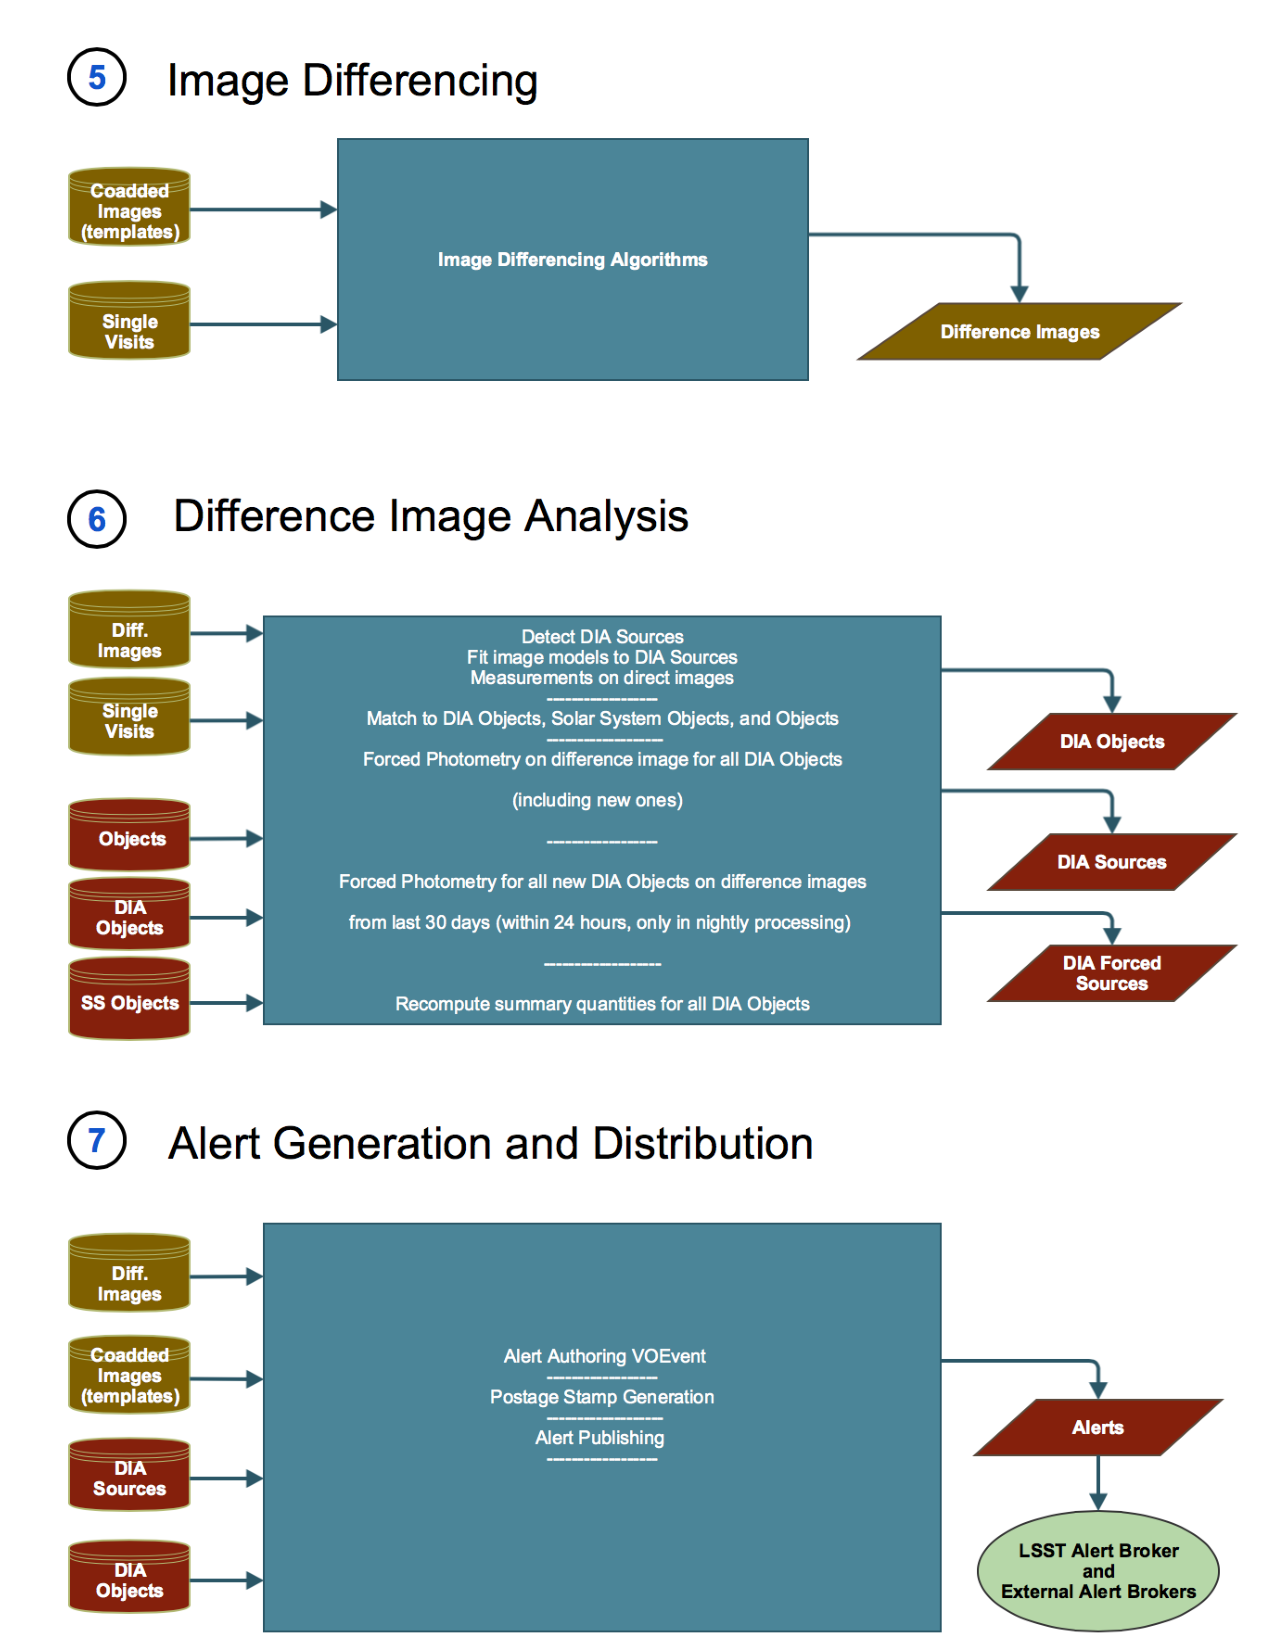
\includegraphics[scale=0.555, angle=0]{gliffy/DifferenceImageProcessing}
    \vskip -0.1in
    \caption{Illustration of the conceptual algorithm  design for Image Differencing, Difference Image
                      Analysis, and Alert Generation and Distribution pipelines. \label{fig:Pipes567}}
\end{figure}

\begin{figure}[!t]
    \centering
    \vskip -2.3in
%    \hskip -0.2in
    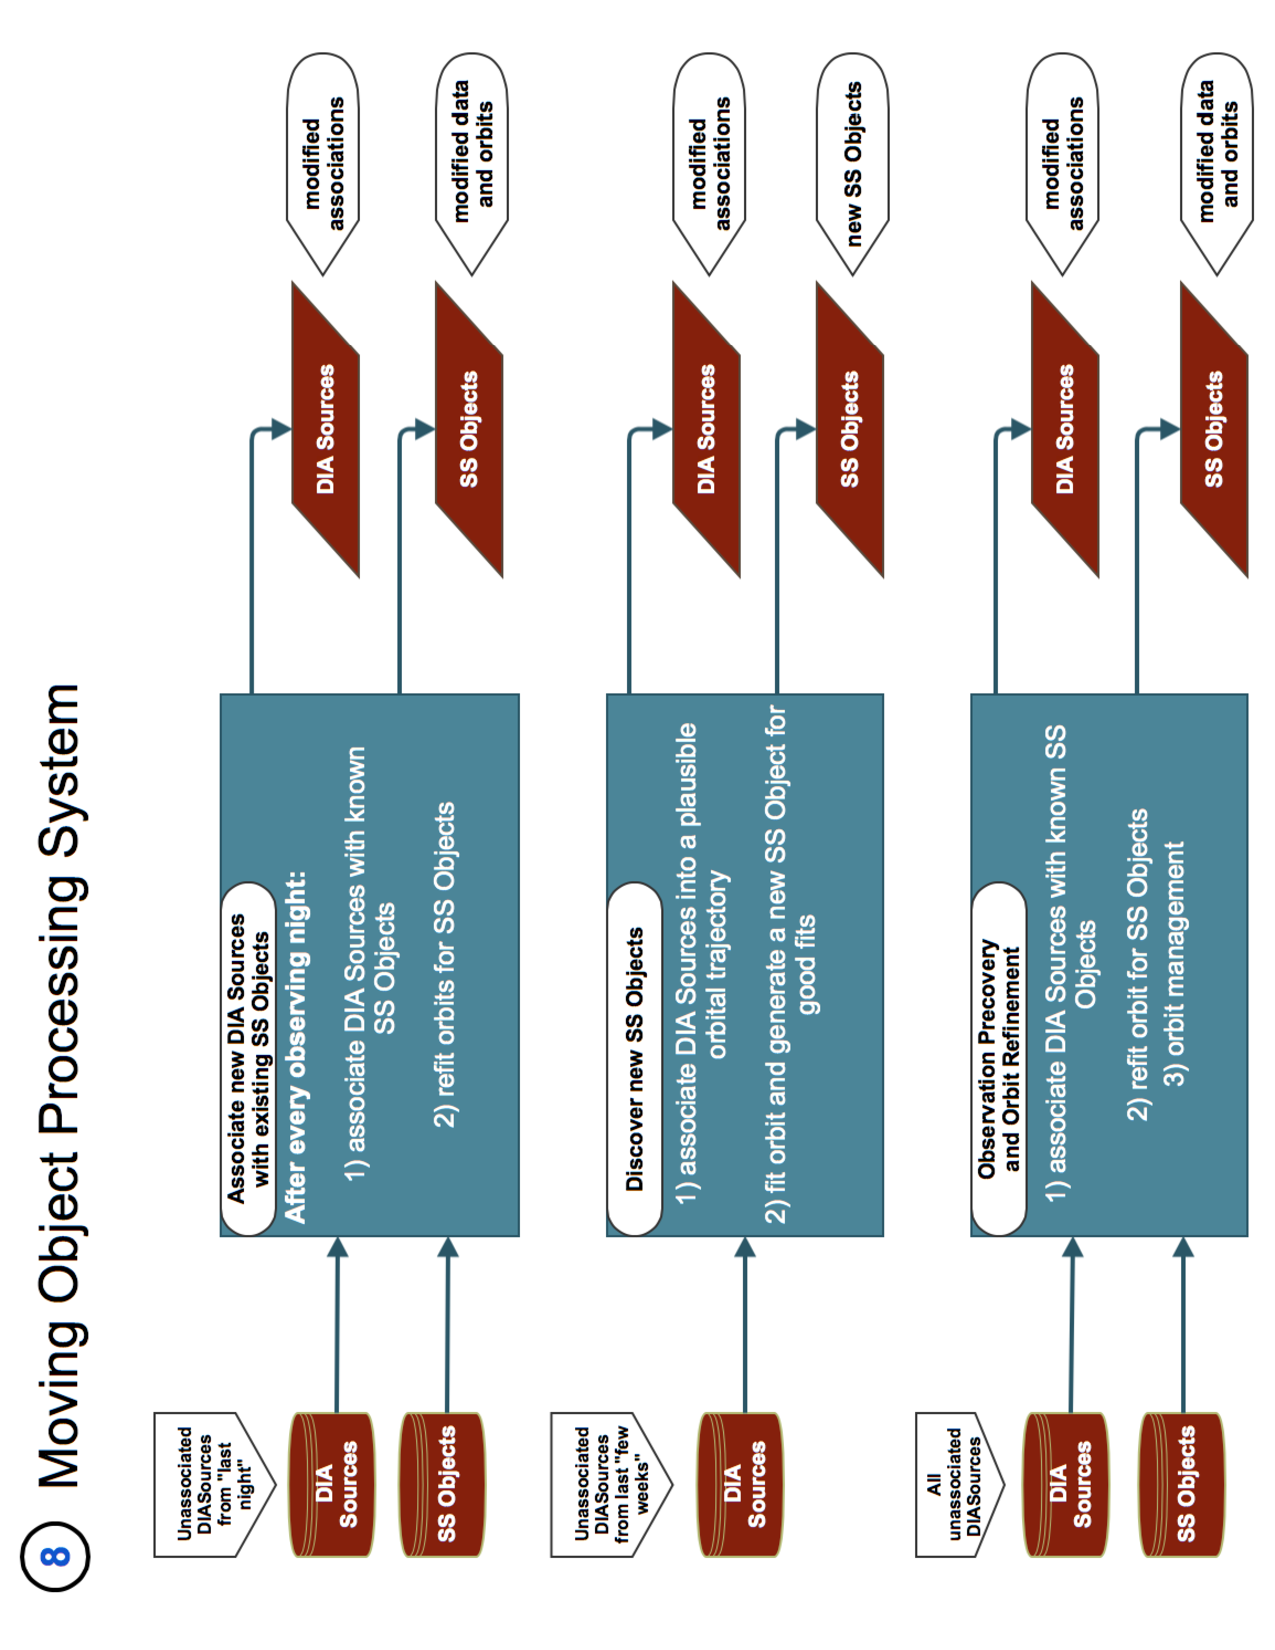
\includegraphics[scale=0.50, angle=270]{gliffy/MOPS-Level0}
    \vskip -0.1in
    \caption{Illustration of the conceptual algorithm design for the Moving Object Processing Software pipeline. \label{fig:Pipe8}}
\end{figure}








\begin{todo}

\clearpage

\section{TODO}

\begin{itemize}

    \item Add Dipole model to DIASource table
    \item References

    \item Selection functions
    \item Understand how to record photometric calibration
    \item Add required accuracy to all tables

    \item Zero-point deltas for different templates
    \item Say more about the image retrieval service

%    \item Mechanisms for updating the document
%    \item Solar System objects in L2
%    \item Solar system object merging with external catalogs
%    \item Deblending, children, etc
%    \item Implement K-T's comments
%    \item Variability characterization
%    \item Crowded field photometry
%    \item Level 3
%    \item Data availability policies
%    \item Colors
%    \item Add canonical band columns
%    \item ID sizes

\end{itemize}

\end{todo}

\end{document}



Unresolved topics:
- maggies
- magnitudes for negative fluxes (and the issue of flux priors)
- how does Alert stream get its QA info? Where are metadata described?
     E.g. the # per CCD, CCD-to-CCD variance, xy cross-correlation
- what about False Source injection?
- how do we know centroids where forced photometry was performed
- do we really need 11 params for PSF model in Source? How about psfFlux and error,
   at the position of centroid (that is, don't refit for the position)


Large edits:
XXX - add dipole fit for DIASources
XXX - redesign of nightly Level 1 db; in sec. 4.2.1 bullet 6 need to mention 12 months window; see also
          bullet 8: the name of db? also, ``full'' light curves? ask Mario...
XXX - redesign of nightly Level 1 db: the main section is 4.3.5 (add Colin's plot?) also, remove reference
          to Level 1 db in 4.5.1
XXX - decide whether to move model description up front, and whether to add anything
XXX - make MOPS diagram and refer to it in Section 4.2.2
XXX - missing DIAForcedSource table; also, can DIASource be DIAForcedSource and ExtendedTable?
        ditto for Source and Forced Source  (look at models plus ``other'' data blocks)
TBD - DIASource: add both light centroid and peak PSF centroid (i.e. mode and mean), trailed source needs centroid
XXX - DIASource: add aperture mags
XXX - fpSky is on direct template image and rename it to fpBkgd
TBD - we need to bring back DIAForcedSource
XXX - adaptive moments in DIASource table (switch to xy), add moments for PSF
XXX - look for spuriousness in LSE-30 (OSS?), add to DIASource table?
XXX - do we want curved trail?   -> footnote
TBD - do we want to fit a gaussian convolved with PSF to each DIASource?

Jim:
- issue of adding Sources, like DIAObjects, to Object list  -> Tucson DMLT

Discussion of DBs, with Andy Salnikov, after reading LDM-135
- ``The LSST baseline database architecture for its real time Alert Production relies on horizontal
time-based partitioning. To guarantee reproducibility, no-overwrite-update techniques combined
with maintaining validity time for appropriate rows are employed.''
      -> what about deleting DIAObjects during MOPS processing?  (for LDM-151, not DPDD)

Mario:
- footnote 45: where is positionMotionLnL?  why are covariances separated if simul fit? Talk to Mario
- flags in DIAObject table: is there any info in other docs to add as a footnote? Talk to Mario
- SSObject table: why two values of MOID? Ask Mario.
- footnote 56: What Gbps WAN do we have now? Talk to Mario


Leftovers from Colin's Minutes for 2016-03-23:
- SAC: Alerts only include footprints for the detection band; is that enough?
- SAC: do we need more than 30 days of precovery fluxes for new DIASources?
        ZI: yes, 30 days is only about two data points in a given band and we don't
                know colors for transients
- ZI: science case for moving variable stars: how do we get LCs and pm/parallax?
- sophisticated matching of DIAObjects to 3 nearest Objects: might want to do
          the nearest star and the nearest galaxy, and the most probable object
- ZI: maggies
- ZI: negative fluxes

Studies for Colissa:
- do we care about direction of NEO motion?
- do we care about curved trails?
- moving variable star: a bias in motion due to flux=const.?
  -- ** other?? **


For Tucson DMLT:

1) Proposal for Nightly Level 1 redesign.
The current baseline is described in DPDD, Section 4.3.5. We will review the
baseline and then discuss the redesign proposal using diagram (attached here):
https://confluence.lsstcorp.org/pages/viewpage.action?pageId=45580703


Tentatively implemented in DPDD.



2) Proposal to perform forced photometry on both difference images
and direct images when Multifit is run in DR Processing.

Tentatively implemented in DPDD.

FYI: the size of ForcedSource table now is 1/4 (=50 TB) of the Source
table size at year 1 and 1/2 (=2 PB) of the Source table size at year 10.


3) How DIAObjects interact with Level 2 DRP processing?  Do we need
to add Sources?

See Jim's note:
https://community.lsst.org/t/unifying-diaobject-and-object-in-drp/716

Also, KT will report about various LL1db vs. DR association issues.



4)  proposal to abolish independent fits of BD galaxy model across bands
        and instead only vary the components’ flux vs. band

what's the plan for arriving to this decision (e.g. process HSC data, or
LSST simulations, or degrade COSMOS data, etc; when?, by ComCam,
DR1, DR11?)


5)  iterative coupled processing of image coaddition and image differencing:
  do we need it or not?


Difference images help to make better coadds by masking moving and transient
objects. But better coadds result in better difference images, which then make
better coadds…


The remaining work in Tucson is to
- submit revised DPDD to CCB: we aim to have finalized DPDD circulated to DMLT
  at least a few days before the f2f in Tucson; we hope to stamp it for CCB there

- in Tucson, Thu/Fri, we will develop plans and diagrams for QA pipelines and for
  calibration product pipelines. We’ll probably use scipi-wg time on Thu for QA pipeline
  discussion, and Fri time for progress on calibration pipelines, as well as discussions
  started by Jim today




KT (from Tucson):
p. 6: is called "calibrated exposure" -> is called a "calibrated exposure"

Section 2.4: move entire section and diagrams to appendix, add forward
reference to LDM-151 for further details on implementation

(Mario) Need to define DIAForcedSource table

Forced DIASources used to update summaries in DIAObjects? Yes

p. 44: fit first to the coadds to initialize the more expensive multi-epoch
fitting -> fit first to the coadds and stored

p. 48: Remove "Two groups of" as well as blue sentence.  Consider saying
explicitly that these variability parameters are per-band.

p. 69: will consider rewriting -> may consider rewriting

----
We will also associate DIASources against the DIAObjects from the latest
DRP and include any match plus its DRP DIASources (and their contents)
in the Alert.  We will still associate against the Live L1 DB and
include the DIAObject match (possibly just-created) from there along
with its associated DIASources.

We will include an extract of the measurements of (all three) Objects in
the Alert as well.

We can save space in L1DB by rolling *versions* of DIAObjects older than
some date to tape (but never the most recent version of a DIAObject,
even if that is old).

DRP DIAObjects will look like L1 DIAObjects (although the exact code may
differ from L1).

Sources are an independent table, not fundamentally associated with
Objects.  Remove Sources from bullet 5 on p. 44; add a footnote
mentioning this.  Nearest Object may be recorded with the Source as a
convenience.
